% Options for packages loaded elsewhere
% Options for packages loaded elsewhere
\PassOptionsToPackage{unicode}{hyperref}
\PassOptionsToPackage{hyphens}{url}
%
\documentclass[
  12pt,
]{article}
\usepackage{xcolor}
\usepackage[top=1.25in, bottom=1.0in, left=1.0in, right=1.0in]{geometry}
\usepackage{amsmath,amssymb}
\setcounter{secnumdepth}{5}
\usepackage{iftex}
\ifPDFTeX
  \usepackage[T1]{fontenc}
  \usepackage[utf8]{inputenc}
  \usepackage{textcomp} % provide euro and other symbols
\else % if luatex or xetex
  \usepackage{unicode-math} % this also loads fontspec
  \defaultfontfeatures{Scale=MatchLowercase}
  \defaultfontfeatures[\rmfamily]{Ligatures=TeX,Scale=1}
\fi
\usepackage{lmodern}
\ifPDFTeX\else
  % xetex/luatex font selection
\fi
% Use upquote if available, for straight quotes in verbatim environments
\IfFileExists{upquote.sty}{\usepackage{upquote}}{}
\IfFileExists{microtype.sty}{% use microtype if available
  \usepackage[]{microtype}
  \UseMicrotypeSet[protrusion]{basicmath} % disable protrusion for tt fonts
}{}
\makeatletter
\@ifundefined{KOMAClassName}{% if non-KOMA class
  \IfFileExists{parskip.sty}{%
    \usepackage{parskip}
  }{% else
    \setlength{\parindent}{0pt}
    \setlength{\parskip}{6pt plus 2pt minus 1pt}}
}{% if KOMA class
  \KOMAoptions{parskip=half}}
\makeatother
% Make \paragraph and \subparagraph free-standing
\makeatletter
\ifx\paragraph\undefined\else
  \let\oldparagraph\paragraph
  \renewcommand{\paragraph}{
    \@ifstar
      \xxxParagraphStar
      \xxxParagraphNoStar
  }
  \newcommand{\xxxParagraphStar}[1]{\oldparagraph*{#1}\mbox{}}
  \newcommand{\xxxParagraphNoStar}[1]{\oldparagraph{#1}\mbox{}}
\fi
\ifx\subparagraph\undefined\else
  \let\oldsubparagraph\subparagraph
  \renewcommand{\subparagraph}{
    \@ifstar
      \xxxSubParagraphStar
      \xxxSubParagraphNoStar
  }
  \newcommand{\xxxSubParagraphStar}[1]{\oldsubparagraph*{#1}\mbox{}}
  \newcommand{\xxxSubParagraphNoStar}[1]{\oldsubparagraph{#1}\mbox{}}
\fi
\makeatother


\usepackage{longtable,booktabs,array}
\usepackage{calc} % for calculating minipage widths
% Correct order of tables after \paragraph or \subparagraph
\usepackage{etoolbox}
\makeatletter
\patchcmd\longtable{\par}{\if@noskipsec\mbox{}\fi\par}{}{}
\makeatother
% Allow footnotes in longtable head/foot
\IfFileExists{footnotehyper.sty}{\usepackage{footnotehyper}}{\usepackage{footnote}}
\makesavenoteenv{longtable}
\usepackage{graphicx}
\makeatletter
\newsavebox\pandoc@box
\newcommand*\pandocbounded[1]{% scales image to fit in text height/width
  \sbox\pandoc@box{#1}%
  \Gscale@div\@tempa{\textheight}{\dimexpr\ht\pandoc@box+\dp\pandoc@box\relax}%
  \Gscale@div\@tempb{\linewidth}{\wd\pandoc@box}%
  \ifdim\@tempb\p@<\@tempa\p@\let\@tempa\@tempb\fi% select the smaller of both
  \ifdim\@tempa\p@<\p@\scalebox{\@tempa}{\usebox\pandoc@box}%
  \else\usebox{\pandoc@box}%
  \fi%
}
% Set default figure placement to htbp
\def\fps@figure{htbp}
\makeatother





\setlength{\emergencystretch}{3em} % prevent overfull lines

\providecommand{\tightlist}{%
  \setlength{\itemsep}{0pt}\setlength{\parskip}{0pt}}



 


% ---- Font: Times New Roman ----
\usepackage{fontspec}
\setmainfont{Times New Roman}

% ---- Line spacing ----
\usepackage{setspace}
\onehalfspacing

% ---- Paragraph spacing ----
\setlength{\parskip}{0.6em}

% ---- Title block ----
\usepackage{titling}
\pretitle{\begin{center}\large\bfseries}
\posttitle{\par\end{center}\vskip 0.4em}
\preauthor{\begin{center}\normalsize\lineskip 0.5em}
\postauthor{\\[0.3em]
  {\small University of California, Santa Barbara} \\[0.1em]
  {\small Department of Economics} \\[0.1em]
  {\small \texttt{coldiron@ucsb.edu}}
  \par\end{center}\vskip 0.2em}
\predate{\begin{center}\normalsize}
\postdate{\par\end{center}\vskip 1em}

% ---- Abstract ----
\usepackage{abstract}
\renewcommand{\abstractnamefont}{\normalfont\bfseries}
\setlength{\absleftindent}{0.5in}
\setlength{\absrightindent}{0.5in}

% ---- Section heading style ----
\usepackage{titlesec}
\titleformat{\section}{\normalfont\large\bfseries}{\thesection}{1em}{}
\titleformat{\subsection}{\normalfont\normalsize\bfseries}{\thesubsection}{1em}{}
\titleformat{\subsubsection}{\normalfont\normalsize\itshape}{\thesubsubsection}{1em}{}

% ---- Graphics and float management ----
\usepackage{graphicx}
\DeclareGraphicsExtensions{.png,.pdf,.jpg}
\usepackage{float}
\usepackage{flafter}
\usepackage[section]{placeins}
\setlength{\textfloatsep}{10pt}
\setlength{\floatsep}{8pt}
\setlength{\intextsep}{8pt}
\renewcommand{\topfraction}{0.9}
\renewcommand{\bottomfraction}{0.8}
\renewcommand{\textfraction}{0.07}
\renewcommand{\floatpagefraction}{0.8}

% ---- Page numbering: centered footer, no header rule ----
\usepackage{fancyhdr}
\pagestyle{fancy}
\fancyhf{}
\fancyfoot[C]{\thepage}
\renewcommand{\headrulewidth}{0pt}
\fancypagestyle{plain}{%
  \fancyhf{}%
  \fancyfoot[C]{\thepage}%
  \renewcommand{\headrulewidth}{0pt}%
}
\makeatletter
\@ifpackageloaded{caption}{}{\usepackage{caption}}
\AtBeginDocument{%
\ifdefined\contentsname
  \renewcommand*\contentsname{Table of contents}
\else
  \newcommand\contentsname{Table of contents}
\fi
\ifdefined\listfigurename
  \renewcommand*\listfigurename{List of Figures}
\else
  \newcommand\listfigurename{List of Figures}
\fi
\ifdefined\listtablename
  \renewcommand*\listtablename{List of Tables}
\else
  \newcommand\listtablename{List of Tables}
\fi
\ifdefined\figurename
  \renewcommand*\figurename{Figure}
\else
  \newcommand\figurename{Figure}
\fi
\ifdefined\tablename
  \renewcommand*\tablename{Table}
\else
  \newcommand\tablename{Table}
\fi
}
\@ifpackageloaded{float}{}{\usepackage{float}}
\floatstyle{ruled}
\@ifundefined{c@chapter}{\newfloat{codelisting}{h}{lop}}{\newfloat{codelisting}{h}{lop}[chapter]}
\floatname{codelisting}{Listing}
\newcommand*\listoflistings{\listof{codelisting}{List of Listings}}
\makeatother
\makeatletter
\makeatother
\makeatletter
\@ifpackageloaded{caption}{}{\usepackage{caption}}
\@ifpackageloaded{subcaption}{}{\usepackage{subcaption}}
\makeatother
\usepackage{bookmark}
\IfFileExists{xurl.sty}{\usepackage{xurl}}{} % add URL line breaks if available
\urlstyle{same}
\hypersetup{
  pdftitle={Twitter and the Politics of the Federal Deficit},
  pdfauthor={Cy Coldiron},
  hidelinks,
  pdfcreator={LaTeX via pandoc}}


\title{Twitter and the Politics of the Federal Deficit}
\author{Cy Coldiron}
\date{2026-04-23}
\begin{document}
\maketitle
\begin{abstract}
Economists and political observers have long noted a recurring pattern
in American politics: politicians change their messaging around the
federal deficit depending on their relative power status---advocating
fiscal restraint (austerity) in opposition, while publicly supporting
fiscal stimulus once in power. This paper examines this claim by
tracking U.S. congressional members' deficit-related tweets between
2017--2023. Using a two-tier dictionary classification method, I
identify tweets referencing the federal deficit and estimate how
deficit-related messaging varies across institutional, legislative, and
fiscal conditions using logistic regression. Deficit-tweeting is low
overall (\textasciitilde0.7\%) but varies significantly depending on a
representative's party affiliation and power status: Republicans tweet
about the deficit five times as often when in the minority, while
Democrats' rates remain comparatively stable across majority/minority
status. Republican leaders' deficit tweeting rates closely track those
of rank-and-file members, while Democratic leadership shows more
heterogeneous patterns. Notably, the fiscal size of legislation has no
measurable effect on deficit tweeting rates. Results confirm that
deficit rhetoric is largely a function of a member's relative political
power and party affiliation---not underlying fiscal
conditions---suggesting that elected officials use deficit messaging to
advance partisan communication goals and legislative agendas.
\end{abstract}


\section{Introduction}\label{introduction}

``It has become standard fare in American politics to watch each party
rail against deficits when they are out of power but hungrily embrace
deficits when in control and able to advance their own agenda.'' ---
\textbf{Kenneth Rogoff}, \emph{Our Dollar, Your Problem}

\subsection{Historical Background of Deficit
Rhetoric}\label{historical-background-of-deficit-rhetoric}

Debates over the size and scope of the federal deficit have been a
central feature of American politics since its inception. Beginning as a
constitutional question in the 1790s, deficits became increasingly
normalized in the 20th century---largely due to the debt-financing of
two world wars,\footnote{Under the gold standard, the government's
  ability to expand the money supply and finance deficits was
  constrained by the amount of gold reserves held by the central bank.
  The U.S. modified the gold standard twice (WWI and WWII) and
  ultimately removed it entirely in 1971 under President Nixon, removing
  this fiscal constraint entirely.} and gradual abandonment of the gold
standard. By the late twentieth century, deficit discourse had turned
uniquely partisan. Political leaders, including then President Ronald
Reagan, attributed the country's economic woes---namely record high
inflation---to the opposition parties' excessive spending policies.
While Reagan advocated, and even campaigned on, reducing the federal
government's size, his eight-year presidency saw a \textasciitilde\$1.7
trillion increase to the national debt.\footnote{Based on U.S.
  Department of the Treasury, \emph{Debt to the Penny} dataset
  (1981--1989). Total debt outstanding rose from approximately \$994
  billion in January 1981 to \$2.7 trillion in January 1989.} Despite
these unprecedented expansionary policies, Reagan was able to depict
himself as a fiscal conservative---showing the potential power of using
partisan rhetoric to shape public opinion. Reagan's successful
rhetorical campaigns greatly influenced the coming decades of political
communication, which has featured increasingly hostile messaging
strategies adopted by both political parties.

Aside from the federal deficit's centrality in American political
discourse, the federal deficit itself has implications for both the
domestic and global economy. In the short run, deficit-spending is
almost always stimulatory, often creating an incentive for the governing
party to spend more to achieve higher growth. However, the debt that
results from repeated deficits can exacerbate longer-term inflationary
pressures, raise borrowing costs and crowd out private investment. This
is not to suggest that deficits are inherently harmful or unnecessary,
or that they have no place in effective economic policy---but rather
that government spending carries meaningful impacts across a range of
economic channels.

Nonetheless, despite both the rhetorical and economic significance of
deficits---there exists little empirical analysis of when and why
deficit rhetoric is used by elected officials. For instance, does
political attention to the national deficit increase in response to
rising debt levels---and is it correlated with other macroeconomic
outcomes? Does an elected official's deficit rhetoric change in response
to their power status or during legislative periods? This paper seeks to
answer these questions. Using elected officials' tweets, I examine the
evolution of deficit rhetoric and analyze how messaging varies across
institutional contexts (who holds power), legislative periods, and
macroeconomic conditions, providing the first large-scale empirical
assessment of how deficit rhetoric functions within the incentive
structure of American politics.

\subsection{Motivation}\label{motivation}

Political discourse can influence public perceptions by directing
attention to certain issues (e.g., health care, immigration) and
influencing how citizens assign responsibility for policy outcomes
(McCombs and Shaw 1972; Iyengar 1991). If this same mechanism applies to
the national debt, then changes to public opinion on deficit spending
may influence legislative agendas---giving political capital for party
leaders to advance policy agendas. For instance, if online deficit
rhetoric impacts public support for fiscal stimulus---then the majority
party's legislative agenda may be forced to change, thereby impacting
the economic trajectory of the country. Deficit rhetoric can also shape
voters' beliefs about the fiscal responsibility of elected officials and
the parties they represent. Thus, political entities that are more
persuasive in their online messaging will potentially have greater
success in electoral campaigns. If this is the case, elected officials
would have reason to communicate about the deficit in such a way that
maximizes success in elections and in passing or opposing
legislation---whether it be consistent with their actual policies or
not. By analyzing the rhetorical patterns of these officials, one can
understand how political actors use the federal deficit to influence
voters' beliefs, and shape public opinion.

\subsection{Why Twitter?}\label{why-twitter}

Twitter (now X)\footnote{Twitter became X in July 2023, following Elon
  Musk's acquisition. This paper uses ``Twitter'' as this study's data
  spans June 2017 to January 2023 (before the acquisition).} is a
uniquely effective medium for this analysis. It is widely and
consistently used by members of Congress and is a direct representation
of each representative's rhetorical intentions. Moreover, tweets are
standardized in format---meaning each post is timestamped, has the same
character constraints, and are tied to verifiable individuals, allowing
for large-scale and reproducible time-series analysis.

Most importantly, tweets reach a far greater audience than other
traditional forms of communication (e.g., floor speeches, hearings)
making them a more impactful communication medium for political
messaging. Based on estimates of average follower count (with median
accounts followed by roughly 100k users) and typical impression rates,
even an average tweet can reach thousands of viewers, with more viral
posts reaching hundreds of thousands (even millions) of people.

As a result, politicians are likely to be especially rhetorically
conscious on Twitter given the platform's broad and immediate public
exposure. In addition, tweets, unlike floor speeches or hearings (which
vary in length and frequency) are published daily by almost all
congressional members. This provides a comprehensive dataset (3.6M
tweets), yielding greater statistical power and enabling stronger
conclusions about key explanatory relationships.

\section{Literature Review}\label{literature-review}

A substantial body of literature has examined various aspects of U.S.
federal deficit spending and the partisan nature of public finance more
broadly (Alesina and Tabellini 1990; Pettersson-Lidbom 2001; Alesina and
Passalacqua 2016). This research provides extensive insight into the
determinants of fiscal outcomes, including how political institutions,
electoral incentives, and partisan control over legislation influence
government spending decisions.

While this research provides extensive analysis of actual fiscal
outcomes, it offers little insight into the political communication
surrounding the national debt itself. To my knowledge, this paper is the
first comprehensive analysis of how politicians' deficit-related
messaging varies with political contexts and fiscal circumstances.

\section{Data}\label{data}

\subsection{Congressional Twitter Dataset
(2017--2023)}\label{congressional-twitter-dataset-20172023}

The dataset used for classifying tweets is Tweets of Congress
(maintained by Alex Litel),\footnote{The data was generated via an
  open-source, serverless application that interfaces with the Twitter
  API, querying for new tweets at the top of each hour; each observation
  is stored as a JSON object with one file per day.} which contains all
tweets (original, retweets, and quoted retweets) from the official
accounts of U.S. congressional members between June 2017 and January
2023.\footnote{Although more recent data (2024--2025) would provide
  greater relevance and utility---especially with the passage of the One
  Big Beautiful Bill (2025)---the cost of X's current API access, which
  changed following Elon Musk's acquisition, is beyond this project's
  financial resources. Under current pricing structures, replicating a
  dataset of similar size (roughly six million tweets) would cost
  between \$30,000 and \$42,000.} This automated pipeline ensures
comprehensive, continuous coverage of congressional Twitter activity
during that period, with accounts updated through routine
synchronization with legislator metadata. For instance, this system
automatically adds newly sworn-in members to the metadata and removes
non-members (i.e., those who lost an election, resigned, etc.)---thereby
reflecting Congress's true composition at each point in time. Notably, I
remove all accounts not directly tied to an individual congressional
member, finalizing the dataset at roughly 3.6 million tweets.\footnote{Excluded
  accounts include party committee handles (e.g., @HouseDemocrats,
  @SenateGOP) and committee-specific accounts (e.g., Armed Services,
  Education). Only accounts directly tied to individual, serving members
  of Congress are retained.}

\subsection{Dictionary-Based Classification of Deficit-Related
Tweets}\label{dictionary-based-classification-of-deficit-related-tweets}

To identify deficit-related tweets, I implemented a two-tier keyword
strategy in Python (pandas). The full code can be seen at the project's
\href{https://github.com/cycoldiron/congress-fiscal-tweets}{GitHub
Repo}.

\textbf{Tier 1 -- Anchor Keywords.} Tweets were flagged as
deficit-related if they contained unambiguous anchor phrases (e.g.,
\emph{``national debt,'' ``balanced budget,'' ``fiscal
responsibility''}). These strong keywords identify explicit deficit
references with high confidence.

\textbf{Tier 2 -- Contextual Expansion.} Tweets containing weaker terms
(e.g., \emph{``debt''}) were only flagged if they co-occurred with
contextual phrases (e.g., \emph{``federal,'' ``budget,'' ``tax,''
``spending''}).

The logic of my labeling framework is to balance the two key
countervailing forces in text classification: precision and coverage.
While a larger keyword dictionary would capture more subtle deficit
references, it would also reduce precision by inflating the number of
false positives. For instance, while including phrases like `trillions
of dollars' may capture references that would otherwise be missed, it
also risks falsely tagging a growing number of unrelated tweets, such as
discussions of income inequality or GDP growth. By contrast, a smaller
dictionary would reduce false positives but would also diminish overall
coverage, leading to more deficit-related tweets going unlabeled.

\subsubsection{Illustrative Example}\label{illustrative-example}

Figures 1 and 2 demonstrate the labeling logic. Rep.~Alexandria
Ocasio-Cortez's reference to ``student loan debt'' is not flagged:
``debt'' is a weak keyword but lacks an accompanying context term. By
contrast, Speaker Kevin McCarthy's reference to the ``national debt''
matches a strong anchor keyword and is thus labeled as
deficit-related.\footnote{Speaker McCarthy's tweet was published outside
  the analytical timeframe (January 2023) but is included here solely as
  an illustrative example of the classification logic.}

\begin{figure}

\begin{minipage}{0.50\linewidth}

\begin{figure}[H]

\centering{

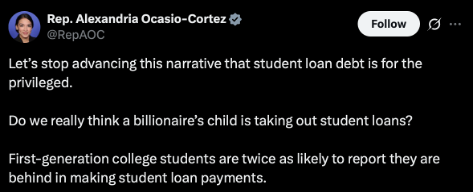
\includegraphics[width=0.85\linewidth,height=1.1in]{../../screenshots/aoc_ss.png}

}

\caption{\label{fig-tweets-1}Rep.~Alexandria Ocasio-Cortez}

\end{figure}%

\end{minipage}%
%
\begin{minipage}{0.50\linewidth}

\begin{figure}[H]

\centering{

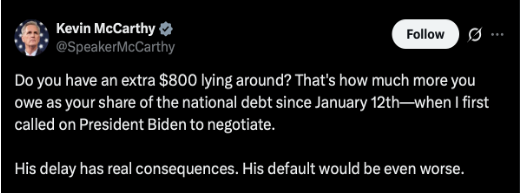
\includegraphics[width=0.85\linewidth,height=1.1in]{../../screenshots/kev_mccarthy_ss.png}

}

\caption{\label{fig-tweets-2}Rep.~Kevin McCarthy}

\end{figure}%

\end{minipage}%

\end{figure}%

\subsection{Measurement Error in Deficit Tweet
Classification}\label{measurement-error-in-deficit-tweet-classification}

While this classification provides simplicity and replicability, it also
introduces potential sources of bias. These fall into two main
categories:

(1) Dictionary Limits: Precision vs.~Coverage

As noted, the challenge in using a dictionary-based method is balancing
precision with coverage. In practice, I adjusted the specificity of both
dictionaries iteratively based on the accuracy of their given
outputs---which I assessed manually by checking the data. While bias in
either direction is statistically possible, my strategy almost certainly
underestimates total deficit rhetoric, since there are theoretically
infinite ways to reference the federal debt.

(2) Variation in Rhetoric and Style

Bias may also arise from differences in rhetorical style across time,
parties, and individuals. For instance, members who consistently use
explicit terms like \emph{``national debt''} are captured reliably,
while those who reference deficits more vaguely or implicitly are
systematically undercounted. If such variation correlates with party or
institutional context (e.g., legislative periods), it could bias
comparisons.

\subsection{Extensions: Supervised Validation and Machine Learning
Approaches}\label{extensions-supervised-validation-and-machine-learning-approaches}

For future research considerations---whether involving similar or
identical data---it is important to consider alternative, complementary
approaches to improve labeling accuracy.

My current strategy relies on a rule-based dictionary method, where I
defined Tier 1 and Tier 2 terms and applied them directly to the full
dataset. While transparent, and easily adjustable, this approach
inevitably misses implicit deficit references and requires subjective
judgment in constructing the dictionaries.

A possible improvement would be to use a supervised dictionary
validation approach. This method first requires manually labeling enough
positive-class instances (i.e., deficit-related tweets), capturing both
explicit and implicit references. Because deficit tweets are rare
(\textasciitilde1--3\% of all tweets), one would need to label roughly
20--30k tweets under an active learning strategy (or 100k+ under random
sampling) to obtain 2--3k positive instances. This threshold aligns with
best practices for addressing class imbalance (Japkowicz and Stephen
2002; He and Garcia 2009). After constructing this training data, one
would build and test multiple dictionary configurations, each with
varying levels of specificity, and then select the configuration with
the highest validated accuracy.

Accuracy would be assessed with two measures:

(1) Coverage: the share of true deficit tweets correctly labeled.

(2) Precision: the false-positive rate.

Selecting the best model would thus require one to determine the ideal
``accuracy'' metric or determining the relative weight of coverage vs
precision. This decision, like my dictionary choices, requires intuition
and could be adjusted based on the researcher's preference.

In sum, a supervised dictionary validation approach would reduce
under-detection of implicit references but would not fully eliminate the
two forms of bias referenced in 3.2. For instance, expanding the
dictionary to improve coverage risks a higher false-positive rate. The
training dataset would capture fewer explicit tweets, and the
best-performing dictionary would detect many of these indirect cases.
Yet the same expansion may also misclassify unrelated tweets, raising
the false-positive ratio. Thus, even if the most comprehensive model
achieved the greatest overall accuracy, the fundamental bias would
persist, albeit at a smaller scale.

\subsection{Institutional, Legislative, and Economic
Covariates}\label{institutional-legislative-and-economic-covariates}

To contextualize congressional tweeting among broader political and
economic phenomena, I integrated a wide set of temporal covariates into
the dataset. Economic indicators---sourced from the U.S. Treasury and
Federal Reserve---include ten-year interest rates, inflation (U.S. CPI
YoY) and multiple measures of federal debt (publicly held debt,
intragovernmental holdings, and total debt outstanding).

Institutional context is captured through variables on presidential
party, House and Senate control, majority and minority leadership, and
whether government is unified or divided, as well as monthly
congressional approval ratings.

Legislative periods are represented by data on major bills from 2017 to
2023 (e.g., CARES Act, PPP, CHIPS Act, IRA). Periods are defined by one
month before and after passage. For instance, the Tax Cuts and Jobs Act
was signed into law by President Trump in December 2017, making its
designated legislative period November 2017--January 2018. Fiscal impact
estimates for each bill come from the Congressional Budget Office (CBO)
and are normalized when included in regression
specifications.\footnote{The fiscal impact of each policy bill is its
  10-year CBO estimate: how much the policy bill is expected to
  contribute to the federal deficit in the ten years following its
  implementation.}

Finally, my research constructs a novel partisanship score formula to
capture the level of partisan division in each legislative period. The
measure is defined as the absolute difference between Democratic and
Republican support rates for a given bill:

\[
\text{Partisanship Score}
= \left|
\frac{\text{Dem Yea}}{\text{Dem Total}}
-
\frac{\text{Rep Yea}}{\text{Rep Total}}
\right|
\]

This score ranges from 0 (perfect bipartisan support) to 1 (completely
partisan support, with only one party voting in favor). For regression
analysis, I normalize the score to standardize across legislative
periods.

\section{Methodology}\label{methodology}

\subsection{Logistic Regression Framework for Deficit
Tweeting}\label{logistic-regression-framework-for-deficit-tweeting}

My research objective is to examine how deficit rhetoric varies with
political, fiscal, and legislative contexts. To assess this
relationship, I estimate a logistic regression model where the dependent
variable is the proportion of a member's tweets in a given month that
are deficit-related.\footnote{Considering the outcome variable is a
  share bounded between (0,1), a traditional linear regression model
  (which allows for values to be negative or greater than 1) would not
  be appropriate. Logistic regression constrains predictions to valid
  probabilities and allows coefficients to be interpreted in terms of
  changes in relative odds of deficit tweeting.} This allows me to
estimate how the likelihood of deficit-related tweeting changes across
political parties, institutional conditions, and legislative
environments.

The unit of analysis is the member-month. For each member \(i\) in month
\(t\), let \(p_{it}\) denote the probability that a given tweet is
deficit-related. The explanatory vector \(X_{it}\) includes party
affiliation, legislative timing indicators, institutional control
variables, and their interactions, as well as normalized measures of
bill partisanship and fiscal magnitude. Models include member fixed
effects (\(\alpha_i\)) and month fixed effects (\(\gamma_t\)), with
standard errors two-way clustered by member and month. Formally,

\[
\log\left(\frac{p_{it}}{1 - p_{it}}\right) = \alpha_i + \gamma_t + \beta X_{it}
\]

Coefficients are exponentiated and reported as odds ratios. Because the
dependent variable is constructed from aggregated tweet counts,
estimates can be interpreted as the effect of these factors on the
underlying probability that a tweet is deficit-related.

\subsubsection{Member and Time Fixed
Effects}\label{member-and-time-fixed-effects}

Member fixed effects absorb differences across legislators and between
parties. For example, Senator Rand Paul tweets far more often than
Senator Ted Cruz, and Republicans, generally speaking, tweet more about
deficits than Democrats. These baseline differences are captured by
\(\alpha_i\), so estimates rely on within-member changes over time.
Moreover, month fixed effects absorb shocks common to all legislators in
a given month. For instance, during COVID-19 legislative periods (i.e.,
CARES Act), both parties reduced deficit rhetoric at similar rates.
Month fixed effects, \(\gamma_t\), ensures that these shared shocks,
such as COVID-19, are not misattributed to partisan--institutional
dynamics.

\subsubsection{Interpreting Odds Ratios and Interaction
Effects}\label{interpreting-odds-ratios-and-interaction-effects}

Each coefficient represents how the odds of tweeting about the deficit
change relative to some baseline condition---which is defined as
Democrats holding the presidency outside of a legislative window (i.e.,
when no major legislation is being voted on). The coefficient on GOP
then captures the baseline ratio of odds between Democrats and
Republicans. Interaction terms assess whether this baseline ratio of
odds (coefficient on GOP) changes as the political context moves from
the baseline circumstance to another political context. Put differently,
the interaction terms examine whether Republicans respond (tweet)
differently than Democrats when the underlying political environment
changes---for example, when moving into a legislative period or when
control of government shifts. If the ratio of odds stays the same when
moving into another political circumstance---i.e., Republicans and
Democrats change their tweeting rates at similar rates---then the
interaction terms will be insignificant.

\subsubsection{Illustration of Interaction Effects in Legislative
Contexts}\label{illustration-of-interaction-effects-in-legislative-contexts}

For example, consider how a single member's behavior changes over time.
Suppose a Democratic member increases their probability of tweeting
about the deficit when moving from a non-legislative period to a
legislative window. The interaction terms in the model ask whether
Republican members change their behavior more or less than Democrats
under the same shift. For example, if the interaction term GOP ×
Legislative Window has an odds ratio less than 1, this indicates that
Republicans change their deficit-related tweeting less than Democrats
during legislative periods, relative to the baseline condition.

Figure~\ref{fig-or-explainer} provides a visual illustration of how the
GOP coefficient defines the baseline Republican--Democrat odds ratio and
how the interaction term modifies that ratio when the political context
changes.

\medskip

\begin{figure}[H]

\centering{

\pandocbounded{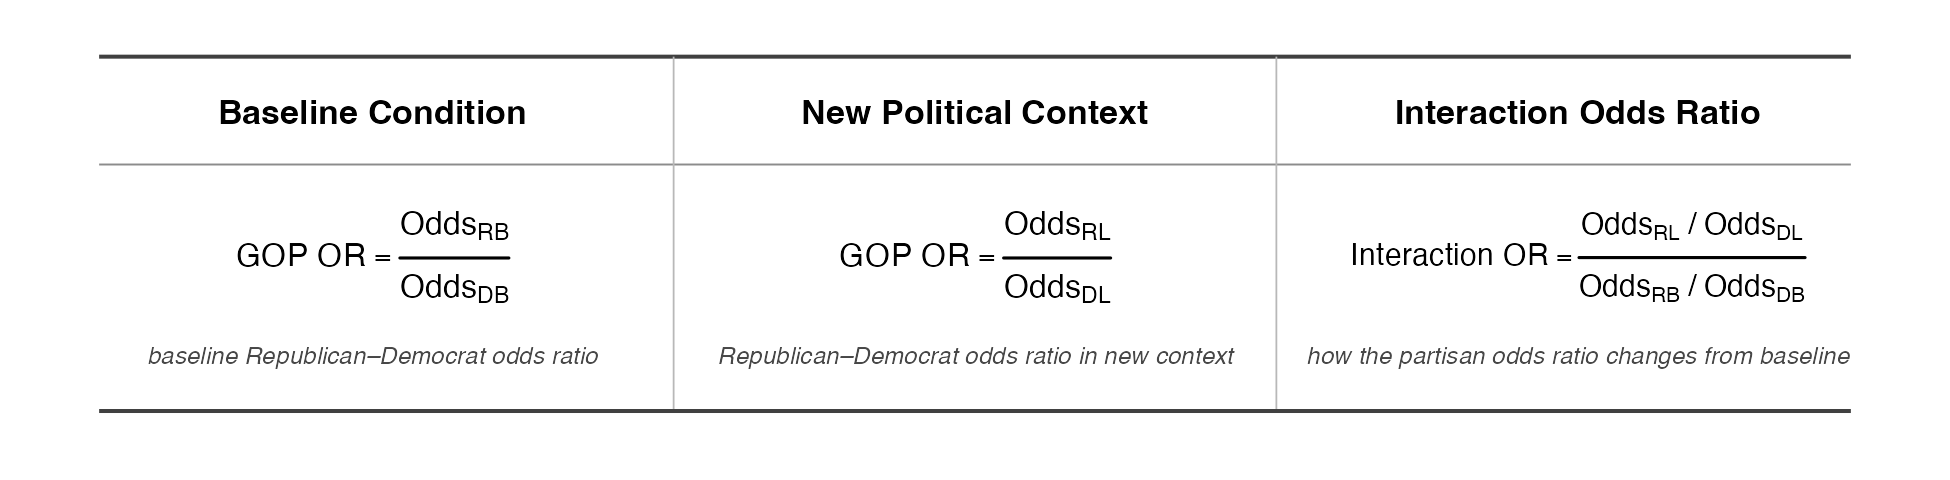
\includegraphics[keepaspectratio]{../../figures/methodology/or_interaction_explainer.png}}

}

\caption{\label{fig-or-explainer}Interpreting the GOP Coefficient and
Interaction Effects.}

\end{figure}%

\medskip

An odds ratio greater than 1 indicates that Republicans increase their
deficit-related tweeting more than Democrats under that condition,
relative to the baseline, while an odds ratio less than 1 indicates that
the Republican--Democrat difference contracts.

\subsection{Sequential Model Specifications and Identification
Strategy}\label{sequential-model-specifications-and-identification-strategy}

My research goal is to understand how deficit rhetoric---specifically
among Democrats and Republicans---changes with varying institutional,
fiscal and legislative conditions. To do this, I estimate a sequence of
specifications that control for these variables in a progressively
specific manner. The baseline model (Regression 1) interacts party
affiliation with legislative windows. Furthermore, it includes
coefficients to describe how this baseline tweeting gap changes with
differing levels of bill partisanship and fiscal impact (CBO estimate of
the bill). Such coefficients help illuminate the relationship---or lack
thereof---between the divisiveness of a bill, or its fiscal impact, and
how members talk about it on Twitter.

The second model (Regression 2) adds a further control by conditioning
on the presidential party (i.e., which party holds the presidency). The
change in coefficient estimates between Regression 2 and the preceding
model indicates that conditioning on presidential power is an important
consideration when analyzing deficit rhetoric. In other words, tweeting
gaps among parties are a function of whose party holds executive power.
Without including this condition, one would improperly interpret the
significance of tweeting differences. Finally, the last specification
(Regression 3) adds further detail by controlling for the composition of
the legislative branch (Congress).

\section{Results}\label{results}

\subsection{Time-Series Trends in Deficit Tweeting
(2017--2023)}\label{sec-macro}

Figure~\ref{fig-timeseries} shows the monthly share of congressional
deficit tweets, by party, from June 2017 to January 2023. Shaded areas
indicate legislative periods -- defined as the month before, during, and
after the passage of a fiscally significant bill. Blue shaded areas
represent legislative periods under a Democratic President (Biden) and
red shaded areas show legislative periods under a Republican President
(Trump).\footnote{Legislative periods exclude small appropriations,
  procedural votes, and commemorations.}

\begin{figure}[htbp]

\centering{

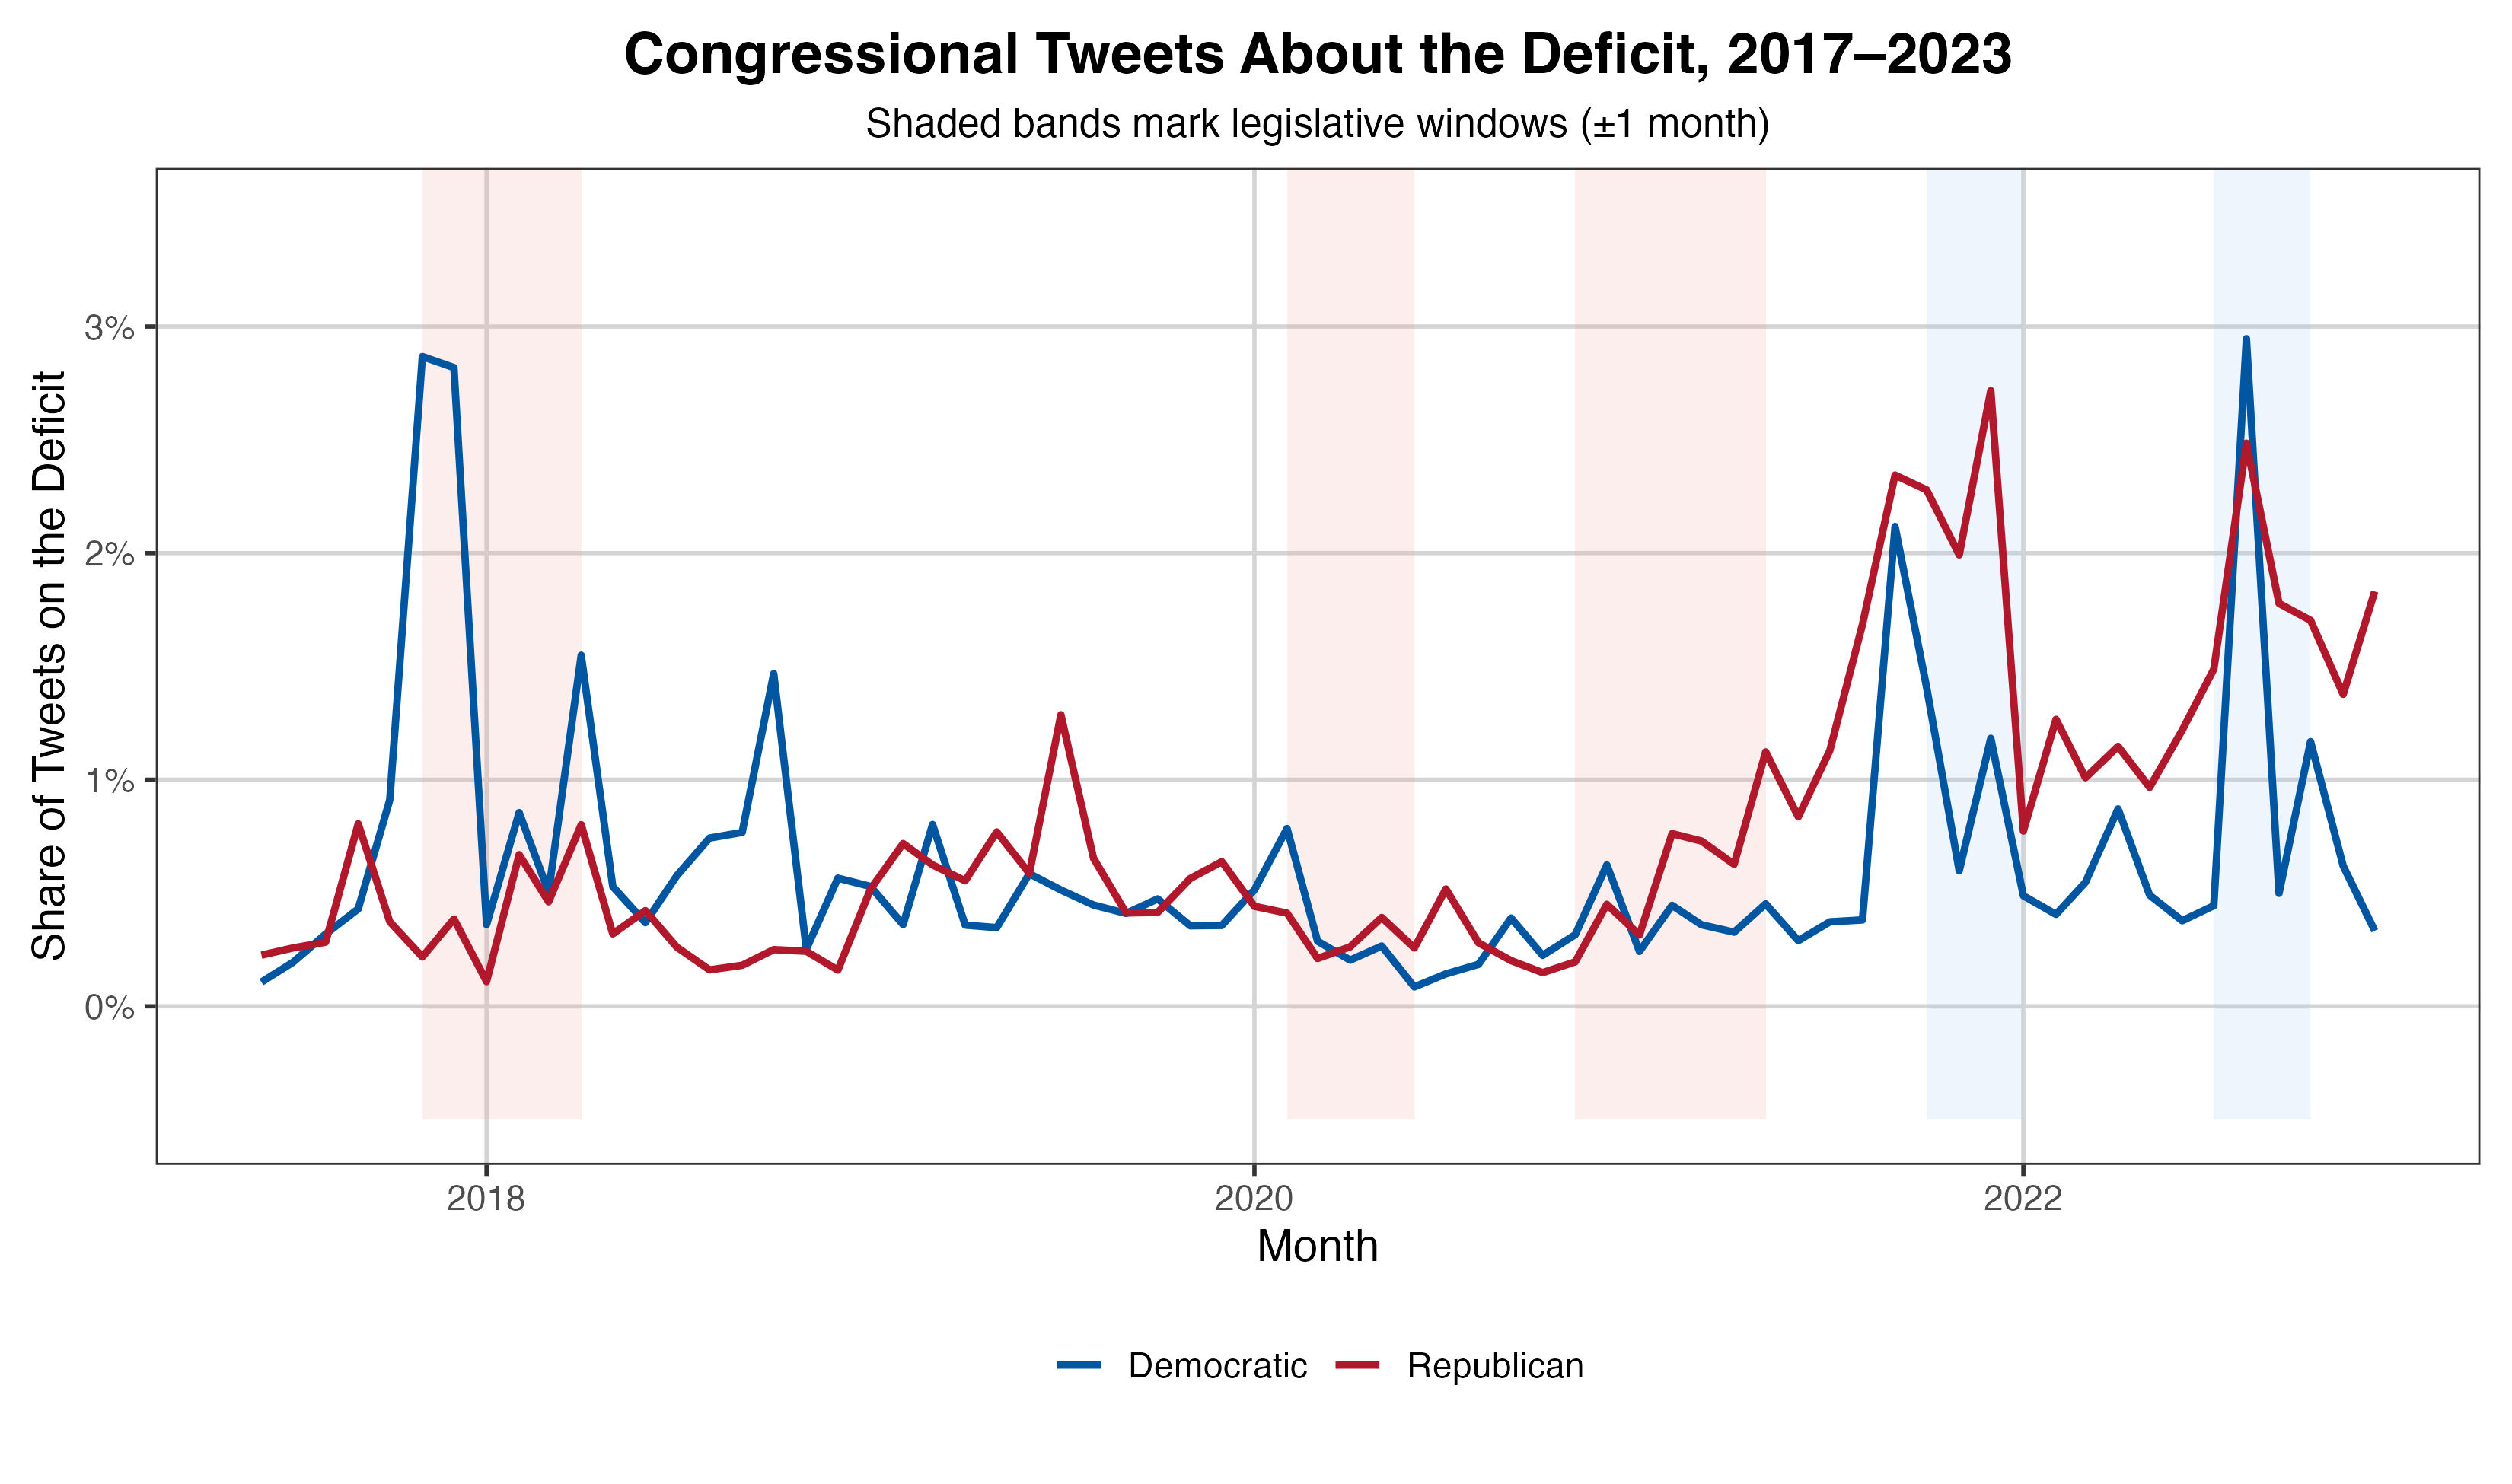
\includegraphics[width=0.78\linewidth,height=\textheight,keepaspectratio]{../../figures/summary/deficit_tweet_share_with_legislation.png}

}

\caption{\label{fig-timeseries}Share of congressional tweets about the
deficit.}

\end{figure}%

The baseline deficit tweeting share for both parties is low, generally
under 1\% when averaged across members over six years, with notable
accelerations occurring around legislative periods. Democratic tweeting
patterns remain relatively consistent across the six years, with three
notable peaks, all during legislative periods: December 2017 (Tax Cuts
and Jobs Act), October 2021 (Infrastructure Investment and Jobs Act),
and August 2022 (Inflation Reduction Act, CHIPS \& Science Act).
Republicans, however, demonstrate consistently higher deficit tweeting
rates as the minority party, as illustrated in the peaks (2022, 2023)
compared to relatively low rates from 2017--2021.

\subsection{Deficit Tweeting and Macroeconomic
Conditions}\label{sec-econ}

Figure~\ref{fig-deficit-vs-cpi}, which plots deficit tweet share against
US CPI inflation (YoY), reveals a relatively strong positive
relationship, as indicated by its large r = .78. There are a few
plausible explanations for this linear relationship. First, the elevated
inflation rates of 2022, peaking at 9.1\% in June (40-year high), may
have increased elected officials' concern about deficit spending. Public
discontent over higher prices may have also pressured representatives to
take a more hawkish approach on federal expenditures.

\begin{figure}[htbp]

\centering{


\includegraphics[width=0.68\linewidth,height=\textheight,keepaspectratio]{../../figures/economic_indicators/deficit_share_vs_inflation_smoothed.png}

}

\caption{\label{fig-deficit-vs-cpi}Deficit tweet share vs.~U.S. CPI
inflation.}

\end{figure}%

Another explanation could be that along with higher inflation, the
significant, and contentious, fiscal legislation being proposed in the
summer of 2022 (e.g., IRA, CHIPS) may have drawn concerns from
representatives, prompting more congressional tweets on the topic.

\subsection{Distribution of Deficit Tweeting Across Members and
Parties}\label{sec-member}

Figure~\ref{fig-member-share-by-party} presents member-level
distributions of deficit tweeting, calculated as the share of each
member's tweets that mention the deficit over the entire period. As
illustrated by the dashed lines (party means), Republicans tweet about
the deficit more frequently than Democrats, with average shares of
0.81\% and 0.62\%, respectively.

Democrats display a relatively compact distribution, with most
representatives falling below 0.7\%. Republicans, however, show far
greater variability within their party. The GOP's right tail
distribution illustrates that, compared to their Democratic colleagues,
a far greater proportion of members tweet about the deficit at much
higher rates, with outliers reaching 4--8\%.

\begin{figure}[H]

\centering{

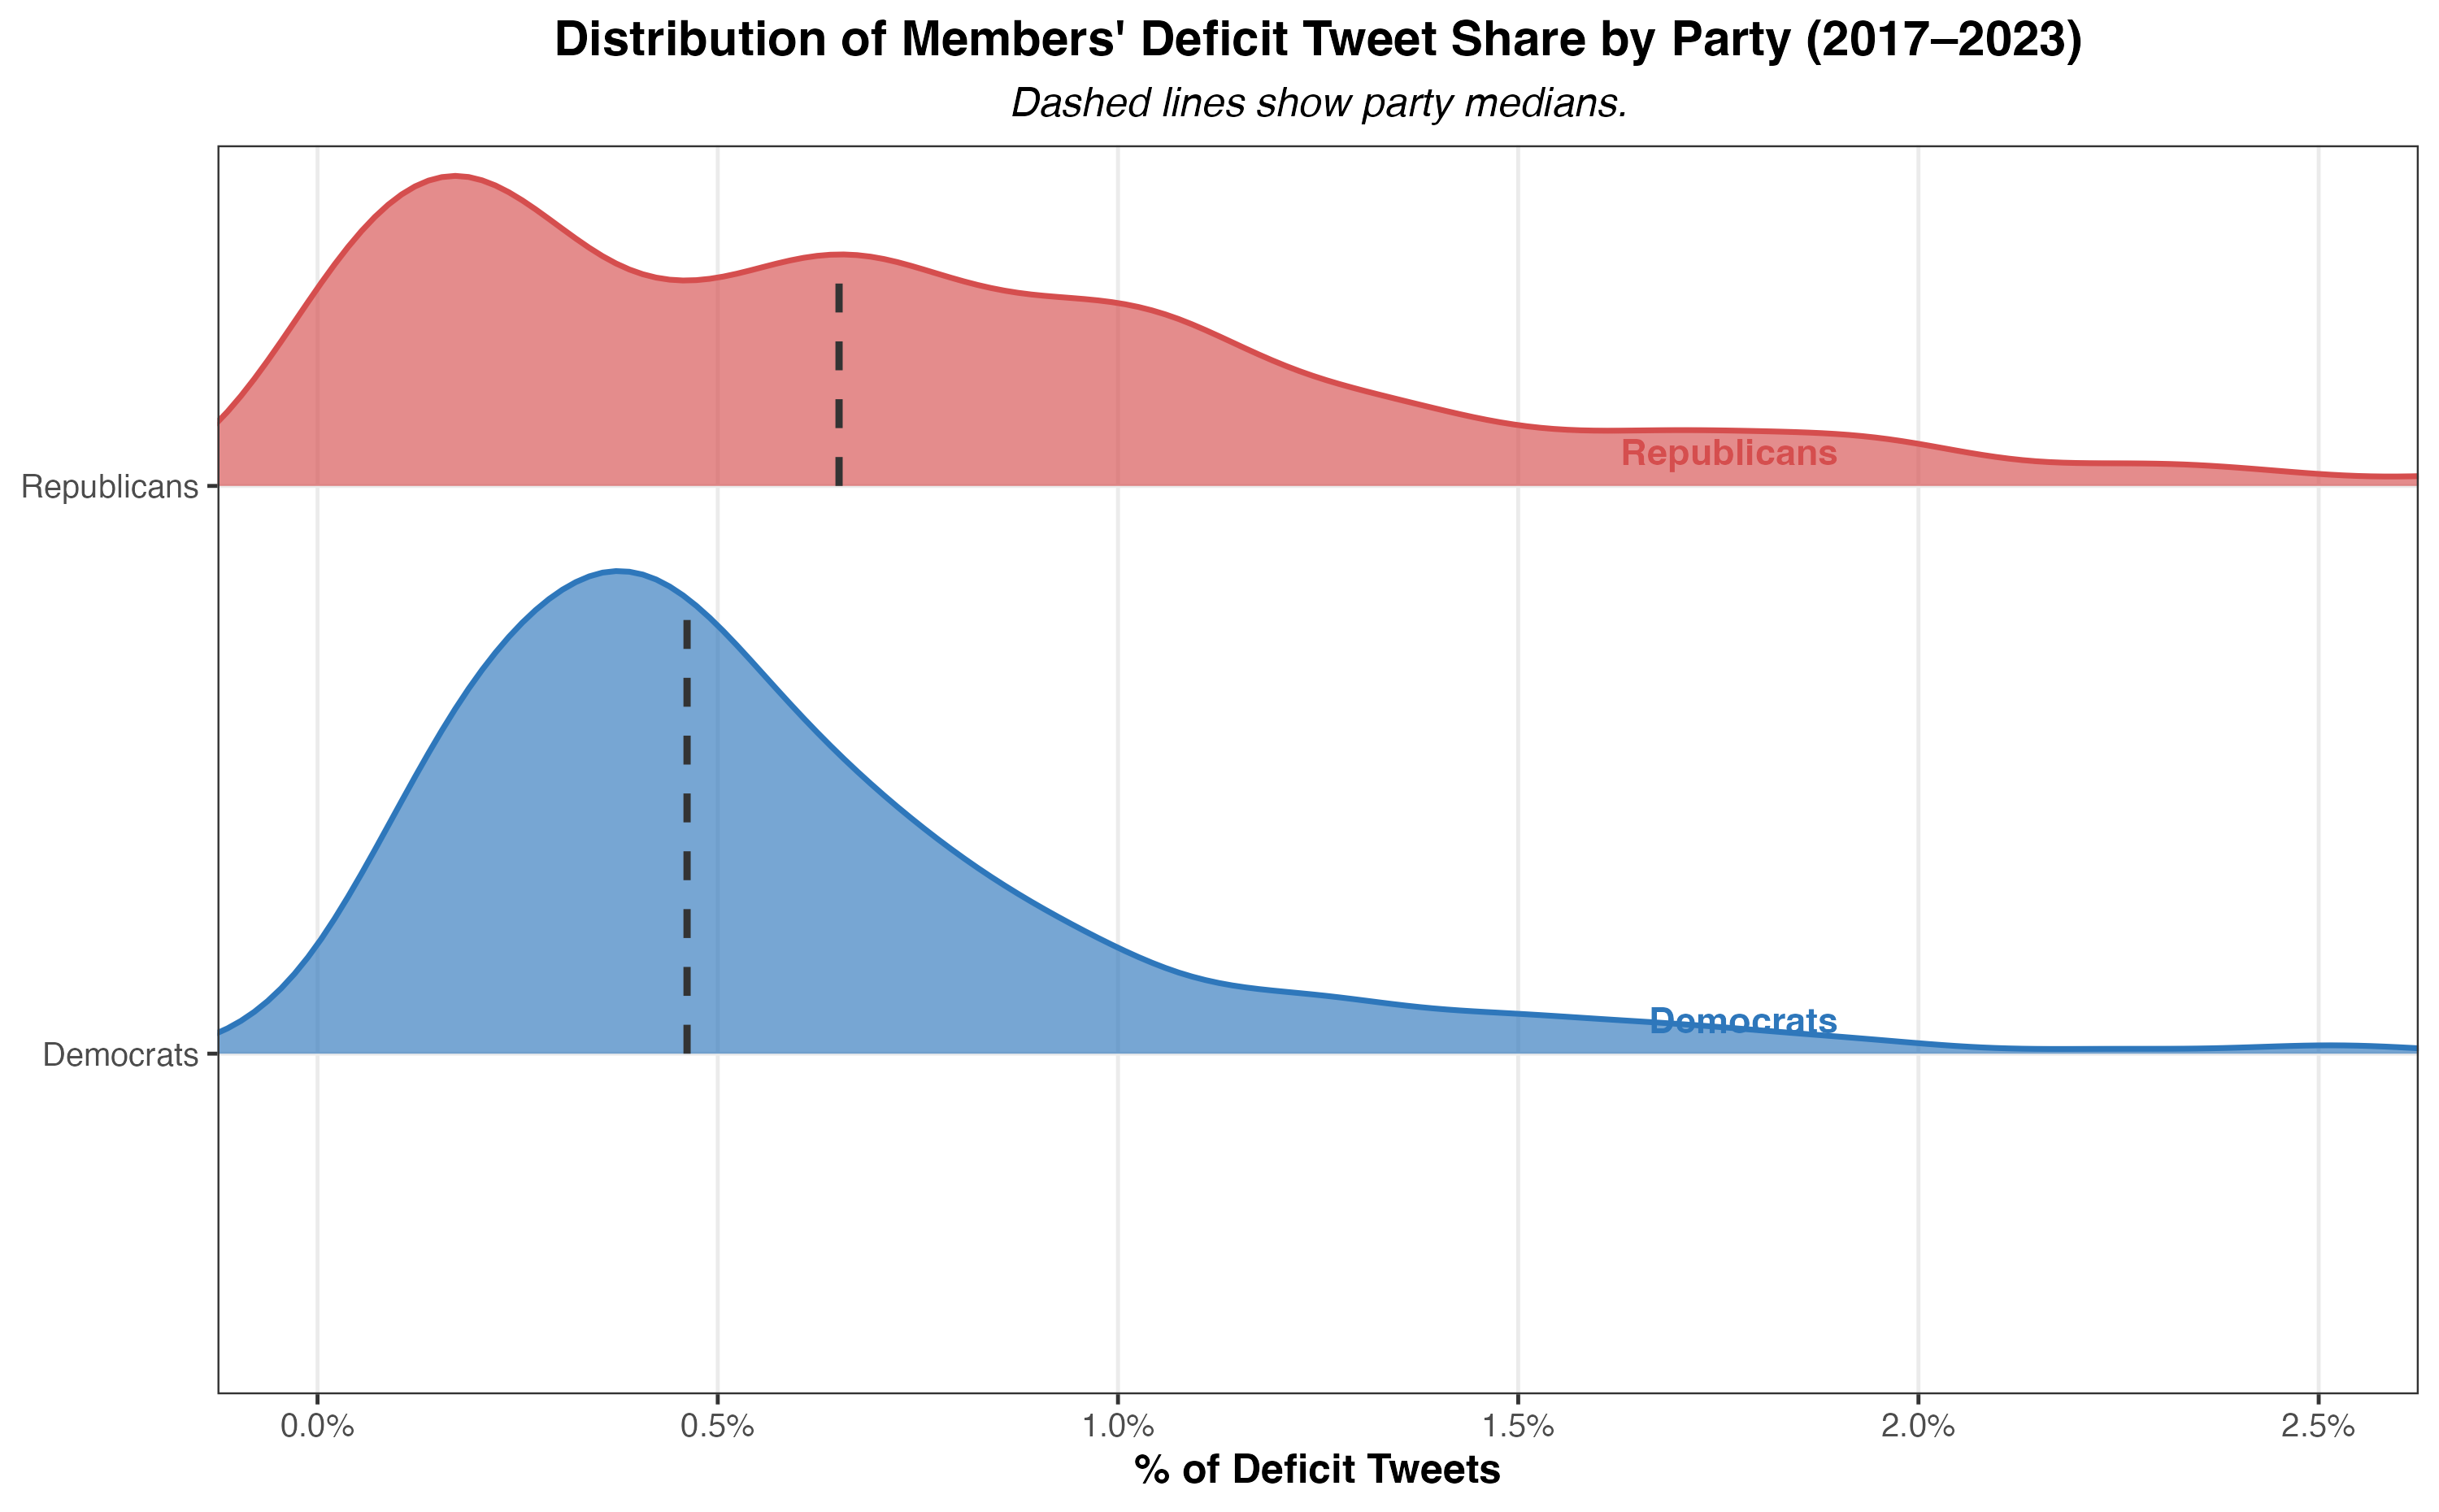
\includegraphics[width=0.72\linewidth,height=\textheight,keepaspectratio]{../../figures/individuals/density_pct_deficit_by_party_overall.png}

}

\caption{\label{fig-member-share-by-party}Share of deficit tweets by
party (member-level distribution). Dashed lines show party means.}

\end{figure}%

\FloatBarrier

Figure~\ref{fig-power-boxplot} breaks down these distributions further
by institutional power status (majority vs.~minority). The left and
right panels compare the distribution when a member's party controls the
presidency (in-power) versus when it does not (out-of-power). For
instance, Democrats would be considered in-power from January 2021 to
January 2023 under President Joe Biden, while Republicans would be
out-of-power during this same period.

\begin{figure}[H]

\centering{

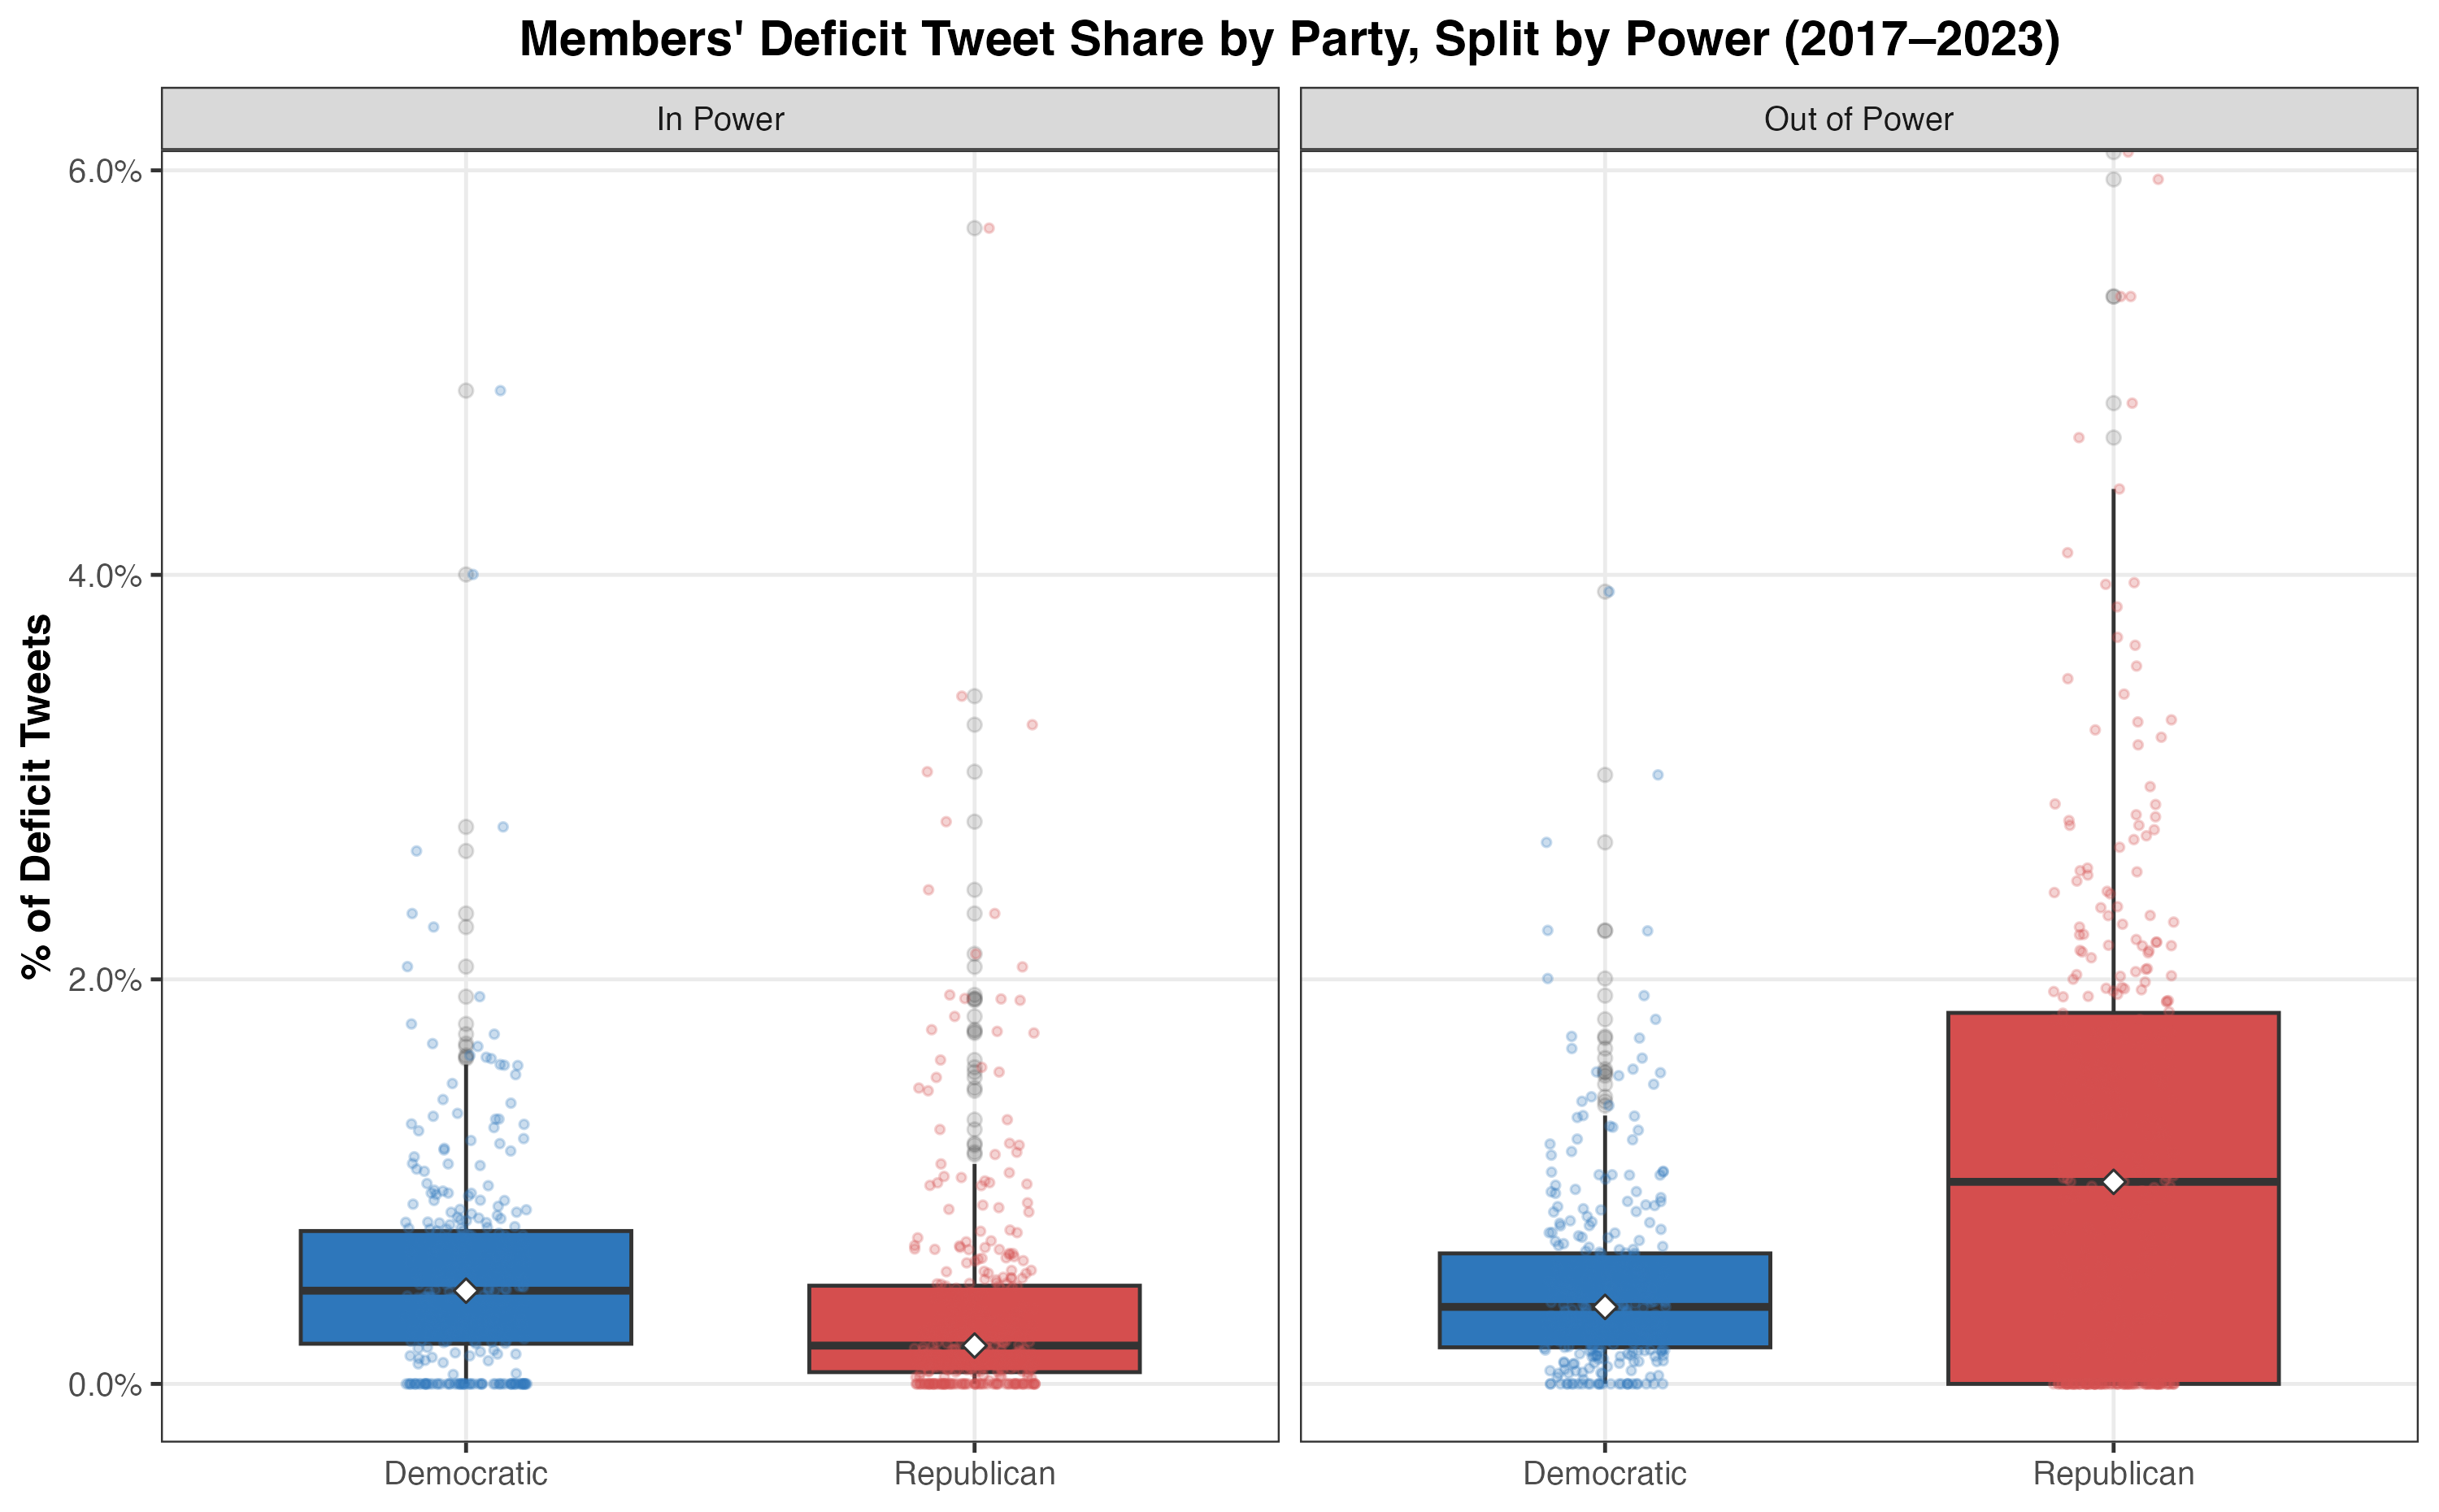
\includegraphics[width=0.72\linewidth,height=\textheight,keepaspectratio]{../../figures/individuals/box_party_split_by_power.png}

}

\caption{\label{fig-power-boxplot}Distribution of deficit tweets by
power (boxplot).}

\end{figure}%

Figure~\ref{fig-power-boxplot} shows a clear asymmetry in Republican
tweeting patterns between these periods. When moving between power
contexts, the Republican median tweet share increases five-fold, from
0.2\% to 1.0\%, and the interquartile range widens from 0.6\% to 1.8\%.
Put simply, Republicans were far more likely to tweet about the deficit
under President Biden than under President Trump. This contrast
illustrates a cohesive shift among Republicans to emphasize the deficit
more when they lack legislative influence. Democrats, by contrast,
remain relatively stable across contexts and in fact demonstrate a
modest increase in spread and averages when in power.

\begin{figure}[H]

\centering{

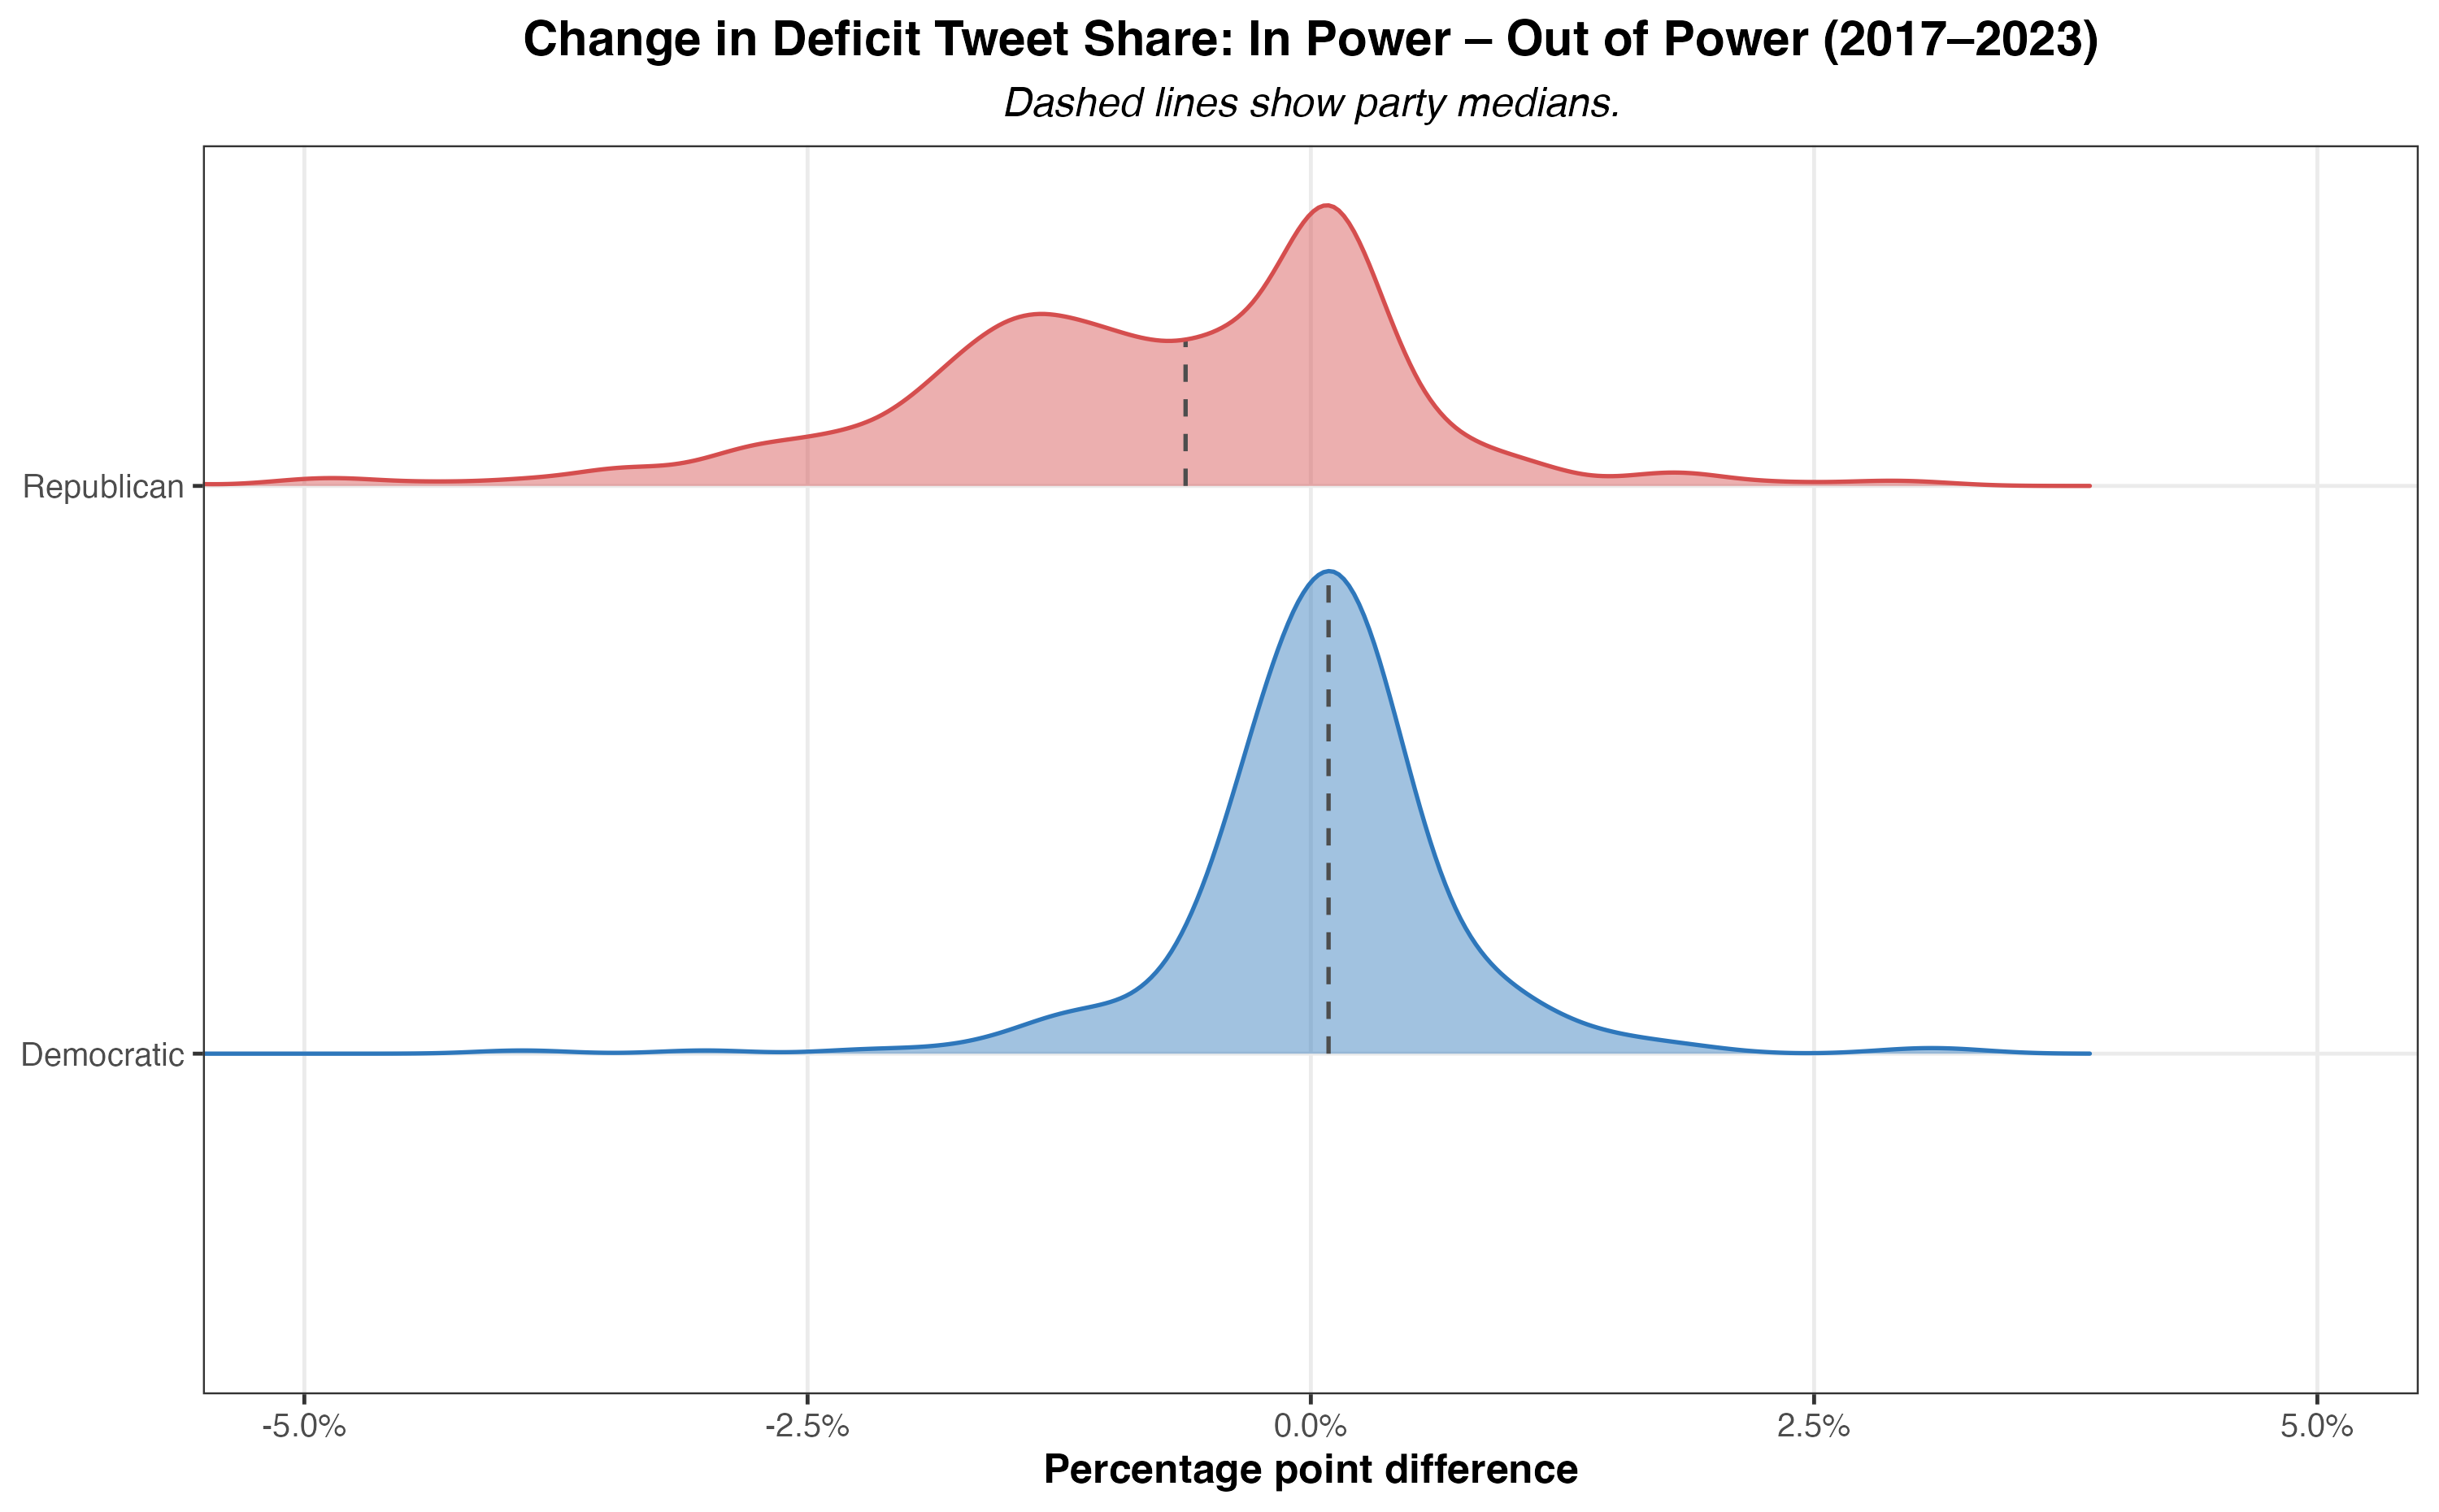
\includegraphics[width=0.72\linewidth,height=\textheight,keepaspectratio]{../../figures/individuals/density_in_minus_out_overlay.png}

}

\caption{\label{fig-inout-shifts}In--out shifts in deficit tweeting
(histogram). Dashed lines show party means.}

\end{figure}%

Figure~\ref{fig-inout-shifts} visualizes these shifts more directly by
plotting the distribution of changes in deficit tweeting when moving
from in-power to out-of-power contexts. The x-axis represents the
difference in deficit tweet share between these two periods for each
member (in minus out). Positive values indicate that a member tweeted
more about the deficit when in power, while negative values indicate
higher tweeting rates when out of power. The GOP's comprehensive party
shift is evident, with the bulk of the party's distribution skewed
negative (i.e., most GOP members tweet more when in the opposition).

\subsection{Deficit Rhetoric Among Congressional
Leadership}\label{sec-leadership}

Table 1 summarizes deficit-tweeting by House and Senate leaders across
majority/minority contexts. Patterns differ by party and chamber, with
the sharpest contrasts in the Senate: Senator Chuck Schumer tweeted
about deficits far more as Majority Leader (4.0\%) than as Minority
Leader (1.0\%), while Senator Mitch McConnell did the reverse (1.9\% in
the minority vs.~0.05\% in the majority). In the House, Representative
Pelosi tweeted about deficits more in the minority (1.1\%) than as
Speaker (0.5\%).

\begin{table}[H]
\centering
\caption{Deficit tweeting by congressional leaders (House and Senate; majority vs. minority roles).}

\includegraphics[width=0.68\linewidth]{/Users/cycoldiron/Desktop/congress-fiscal-tweets/figures/leadership/leader_deficit_tweets.png}
\end{table}

Notably, Representative McCarthy has relatively few tweets (762).
Because leaders often switch or add handles when roles change, the data
collection process may have failed to include relevant accounts. Thus,
McCarthy's deficit tweet share should be interpreted cautiously.

While the preceding analysis covers broader party-level trends,
exploring individual leaders' tweeting patterns provides insight into
how key political figures communicate about the deficit in varying
institutional contexts. Considering the legislative and electoral
significance of these figures, their messaging strategies are more
influential and calculated than those of rank-and-file members. For
instance, party leaders may use specific communication strategies around
legislative periods to catalyze or bar the passage of key bills.
Examining these trends can therefore help illustrate the degree of
strategic communication employed by top legislators, and by extension
--- the party they represent.

Consider the differences in tweeting patterns among the two parties' top
legislators. First, for Democrats, the divergent tweeting patterns of
Speaker Pelosi and Senator Schumer suggest a weak intra-party alignment
in messaging. These patterns are consistent with the broader Democratic
caucus, which shows no discernible difference in deficit tweeting
between power contexts (as shown in Figure~\ref{fig-power-boxplot} and
Figure~\ref{fig-inout-shifts}). The Republican party, however, is more
responsive to changes in their power status. Senator McConnell's
increase in deficit tweeting in out-of-power contexts mirrors the
broader Republican trend illustrated in Figure~\ref{fig-inout-shifts}.
Furthermore, McConnell's tweeting patterns confirm long-held conceptions
about his communication and political style, which emphasizes
unrelenting opposition to Democratic fiscal policies (MacGillis 2014;
Hacker and Pierson 2016).

\FloatBarrier

\subsection{Deficit Tweeting Within Legislative
Windows}\label{sec-leg-context}

\begin{table}[H]
\centering
\caption{Deficit share within legislative windows, by party.}

\includegraphics[width=0.65\linewidth]{/Users/cycoldiron/Desktop/congress-fiscal-tweets/results/good_summary_tables/tweetlevel_deficit_share_by_party.png}
\end{table}

Table 2 reports the conditional share of tweets mentioning the deficit
within ±1-month windows around major bills, split by party (with a
pooled/overall column for reference). At baseline, Republicans tweet
about the deficit more often (0.8\%) than Democrats (0.6\%) -- a gap
that persists across most legislative windows. During the Inflation
Reduction Act (2022) and CHIPS Act (2022) periods, Republicans' tweets
accelerated, with deficit mentions at nearly 2.0\%, compared to 1.3\%
among Democrats. However, the TCJA (2017)---a partisan GOP tax cut---is
a noticeable and stark exception. During these three months, the
Democrats' deficit share spikes to 2.0\%, while the Republicans' share
falls to just 0.2\%, reflecting a partisan realignment around a highly
divisive bill. In contrast, during the COVID relief period in 2020 -- a
non-partisan voting context -- both parties converged at very low levels
(0.3--0.4\%).

\FloatBarrier

\subsection{Regression Results: Institutional and Legislative
Interactions}\label{sec-reg-viz}

The following regression models offer a structured approach to examining
how institutional, fiscal, and partisan contexts affect the likelihood
of congressional deficit tweeting. Each model includes interaction
coefficients of the general form GOP × Conditioning Variable, indicating
whether the baseline Republican--Democratic difference changes under
specific conditions.

\begin{table}[htbp]
\centering
\caption{Regression 1: Legislative windows.}

\includegraphics[width=0.80\linewidth]{/Users/cycoldiron/Desktop/congress-fiscal-tweets/results/good_regression_tables/r3_legislative_windows_main.png}
\end{table}

The baseline model, Table 3, examines partisan differences in
legislative periods without conditioning on institutional control. The
non-significant results suggest that, when averaged across both
Democratic and Republican presidencies, legislative windows themselves
do not systematically impact the partisan gap in deficit tweeting.

\begin{table}[htbp]
\centering
\caption{Regression 2: Majority context (presidency).}

\includegraphics[width=0.80\linewidth]{/Users/cycoldiron/Desktop/congress-fiscal-tweets/results/good_regression_tables/r5_majority_context_main.png}
\end{table}

Table 4 controls for presidential party by adding an indicator for
serving under the out-party president (GOP under a Democratic president;
Democrats under a Republican president) and by interacting it with
Legislative window, plus the three-way term GOP × Legislative window ×
Minority presidency. These terms let the GOP--Dem deficit-tweeting gap
differ under Democratic vs.~Republican presidents and specifically
during legislative months.

Republicans' odds of tweeting about deficits are nearly double (OR =
1.87) when not holding the presidency (i.e., Joe Biden is President)
compared to Democrats under the same condition. In contrast, GOP ×
Legislative window (OR= 0.38) highlights that under a Republican
presidency, the partisan gap narrows during legislative months---the
odds of the GOP tweeting are 62\% lower than those of Democrats. In
other words, Republicans are far less likely to discuss the deficit when
their party holds the executive branch. This pattern aligns with
Figure~\ref{fig-timeseries}, which shows that Republican tweeting
contracts while Democratic tweeting spikes as Congress passed the Tax
Cuts and Jobs Act in late 2017. However, the three-way interaction
coefficient GOP × Legislative window × Minority presidency reveals a
reversal of this trend (OR= 4.24). Under a Democratic presidency (Joe
Biden), Republicans' odds of tweeting are more than four times higher
than those of Democrats in the same condition.

\begin{table}[htbp]
\centering
\caption{Regression 3: Majority context --- chamber and presidency combinations.}

\includegraphics[width=0.80\linewidth]{/Users/cycoldiron/Desktop/congress-fiscal-tweets/results/good_regression_tables/r6_majority_context_combos.png}
\end{table}

Table 5 examines how the tweeting gap changes by who controls
congressional and executive branches. A GOP trifecta means Republicans
held the presidency, House, and Senate simultaneously---a condition they
held from 2017 to 2019. The model includes indicators for these control
combinations: the baseline is Democrats outside legislative windows when
their party controls no institution (minority in both chambers and not
holding the presidency). This context would describe Democrats, between
2017 and 2019, in non-legislative periods (i.e., not during Tax Cuts and
Jobs Act).

GOP × Legislative window (OR = 0.31) indicates that during legislative
months, when holding a trifecta, Republicans' odds of tweeting are 69\%
lower than Democrats. The Tax Cuts and Jobs Act (2017)---a legislative
window under a GOP trifecta---is an illustration of this condition.
However, once conditioning on a Democratic trifecta, this effect
reverses. Relative to the baseline condition (a GOP trifecta),
Republicans' odds of deficit tweeting are seven times higher than those
of Democrats in the same context. The juxtaposition of these two
coefficients (OR = 0.31) versus (OR = 7.00) illustrates that legislative
timing by itself is not a determinant of tweeting gaps---but who governs
is. Under Democratic control (i.e., 2021--2023), Republicans accelerate
deficit rhetoric during legislative months, while under the GOP trifecta
(i.e., 2017--2019), they significantly reduce deficit tweeting
frequencies.

\subsubsection{Effects of Bill Partisanship and Fiscal
Magnitude}\label{sec-bill-partisanship}

Across all three specifications, the coefficients for Fiscal magnitude
(z) are statistically insignificant (\textasciitilde1.0). These
coefficients, based on a normalized measure of a given bill's 10-year
CBO estimate, suggest that the fiscal consequences of policy do not
systematically impact partisan tweeting gaps.

Bill partisanship (z), however, shows significant contractions in the
GOP-Dem tweeting gap once institutional control is included (OR
\textasciitilde{} 0.50). In other words, for each one-SD increase in a
bill's partisanship score, the GOP-Dem gap contracts by roughly half.
Notably, because these variables are continuous (i.e., z-scores), the
coefficients represent slopes rather than a baseline-specific effect.
For example, in the context of bill partisanship, if Republicans are
twice as likely as Democrats to tweet at z = 0 (OR = 2.0), that gap
narrows to parity at z = 1 (OR = 1.0).

\FloatBarrier

\section{Discussion}\label{discussion}

\subsection{Summary of Empirical Patterns in Deficit
Tweeting}\label{summary-of-empirical-patterns-in-deficit-tweeting}

My research finds that deficit rhetoric on Twitter among U.S.
congressional members is low---fluctuating between averages of .5\% to
2\% throughout the six-year periods (or 5-20 ``deficit tweets'' per 1000
tweets). However, my results highlight significant and important
nuances. Specifically, I find that variation in deficit tweeting is
strongly tied to two factors---relative institutional power and
legislative timing. I also find that deficit rhetoric is not tied to the
fiscal magnitude of policy bills; that is, tweeting rates are
uncorrelated with the long-term fiscal impact of legislation (measured
by its 10-year CBO estimate).

As noted, institutional power---whether a member's party holds
congressional and/or executive control---is a key determinant of deficit
tweeting among Republicans, but not Democrats. It also helps to explain
significant variations in tweeting gaps among the parties. For instance,
Republicans' deficit rhetoric increases five-fold when transitioning
into out-of-power contexts (holding all other factors constant) while
Democrats' rates remain constant throughout. Republican leaders mirror
the trends of their rank-and-file members (by increasing deficit
tweeting in out-of-power contexts), while Democratic leaders show no
discernible pattern in contextual tweeting among each other.

Regression analysis also indicates that legislative windows influence
deficit tweeting only after conditioning on presidential and/or
congressional control. In other words, Republican--Democrat tweeting
differences only change once one considers who is in power. The partisan
tweeting gap contracts in legislative months where Democrats hold the
presidency.

These results suggest that, for Republicans, deficit rhetoric functions
as a context-dependent communication resource. Members will emphasize
the deficit when political accountability is externalized---that is,
when Democrats hold power. However, once Republicans move into periods
of legislative power (i.e., political accountability is internalized),
they tend to diminish their deficit rhetoric significantly.

\subsection{Deficit Rhetoric is Independent of Fiscal
Conditions}\label{deficit-rhetoric-is-independent-of-fiscal-conditions}

Results show no discernible relationship between the fiscal magnitude of
legislation and deficit tweeting: members do not increase references to
the deficit in legislative periods that are characterized by large
spending. For example, deficit tweeting is the same for policy bills
that have a low fiscal impact (such as the Inflation Reduction Act) and
legislation with high fiscal impact (such as the Tax Cuts and Jobs Act).
Notably, the fiscal magnitude of bills does not predict tweeting gaps
once institutional controls are included.

One would assume that deficit rhetoric should derive from the very thing
it references---the federal deficit. My research, however, suggests that
no such relationship exists. This is an important relationship, or lack
thereof, that stakeholders (voters, journalists, and forecasters) should
understand: deficit rhetoric, most of the time, should not be
interpreted as a direct proxy for fiscal concern, but rather as a
reflection of a representative's power and political incentives.

\subsection{Partisan Asymmetry and Message
Coordination}\label{partisan-asymmetry-and-message-coordination}

Beyond these aggregate patterns, my findings highlight important
asymmetries between political parties' communication patterns. First,
Republicans exhibit greater sensitivity to power status; that is, their
deficit tweeting rates fluctuate significantly depending on who controls
Congress and the presidency.

The second asymmetry which warrants consideration, is the difference in
coordination and alignment among party leaders and rank-and-file
members. Republican leaders, compared to their Democratic counterparts,
demonstrate a greater degree of both partisan messaging and uniformity
with their members. For instance, consider Representative Paul Ryan---a
self-described fiscal conservative, Speaker of the House from
2017--2019, and a central political figure in modern discourse
surrounding the national deficit. While Ryan frequently branded himself
a ``deficit hawk,'' his public deficit messaging was minimal during
unified GOP control as Congress advanced the Tax Cuts and Jobs Act,
which the CBO estimated would add roughly \$1.5 trillion to the debt
over ten years. In short, Ryan rarely emphasized the deficit while
orchestrating a major deficit-increasing legislative agenda. Ryan's
self-contradictory tweeting behavior is emblematic of the claim I have
highlighted in this section: deficit messaging, especially for
Republicans, is not a proxy for genuine fiscal worries, but is a
reflection of a representative's political incentives.

Furthermore, as the only Republican to serve as both the minority and
majority leader, Mitch McConnell serves as an effective illustration of
a representative cyclically aligning their rhetoric to serve political
means. As Table 1 shows, during his four-year role as majority leader,
McConnell tweeted about the deficit just three times out of 5,622 total
tweets---a staggering 0.05\% deficit-tweet rate. This stands in sharp
contrast to his tweeting patterns as the minority leader, under
President Joe Biden, where McConnell's deficit tweeting rates increased
to 1.89\%---a 38-fold increase. Senator McConnell---the spokesperson for
the Republican party---made a conscious effort to vastly alter his
deficit-rhetoric during his time in the opposition. And the broader
Republican party followed in unison with his messaging goal---increasing
deficit tweeting rates significantly in minority contexts. Taken
together, these rhetorical trends suggest a top-down messaging dynamic
among Republicans: party leaders establish rhetorical cues that are
consequently adopted by rank-and-file members.

By comparison, the Democratic party illustrates both less intra-party
coordination and less sensitivity to changes in their relative power.
For example, the diverging tweeting patterns of Speaker Pelosi and
Senator Schumer suggest a comparatively weaker intra-party alignment in
messaging. Speaker Pelosi tweets at higher rates in the minority versus
majority (1.11\% vs.~0.50\%), while Senator Schumer tweets at
significantly higher rates in the majority (1.03\% vs.~4.00\%). My
results suggest that Democratic messaging is far more heterogeneous at
both the leadership level (Pelosi and Schumer), and among rank-and-file
members themselves. Overall, Republicans---intentional or not---are far
more successful in articulating organized and context-specific
messaging.

\subsection{The Political Incentives of the Federal Deficit: Blame
Avoidance and Ideological
Signaling}\label{the-political-incentives-of-the-federal-deficit-blame-avoidance-and-ideological-signaling}

The bulk of this paper thus far has dealt with objectively describing
the nature of deficit rhetoric among U.S. congressional members. My
analysis naturally brings about a key question: what motivates
politicians' deficit-related messaging on Twitter? While the precise
motivations underlying elected officials' communication choices cannot
be directly observed---i.e., one cannot know the reasoning behind every
tweet---the systematic patterns in the data provide a constructive
foundation for interpretive analysis.

The most plausible explanatory factor driving deficit rhetoric is the
political incentive to externalize fiscal blame on the opposing party.
Minority parties, while lacking any real legislative, governing, or
subpoena power, have the capacity to frame the opposing party as
fiscally irresponsible in hopes of improving their popularity or
electoral prospects. This political incentive weakens once a party gains
legislative control as it no longer becomes politically advantageous to
discuss---or in this case, tweet---about the federal deficit.

Such an explanation is consistent with Kent Weaver's political theory of
blame avoidance. Given that voters are more sensitive to negative
outcomes than positive ones (negativity bias), Weaver observes that
politicians are motivated to be `blame minimizers', not `credit
maximizers'. Under Weaver's framework, governing parties would therefore
have an incentive to suppress deficit rhetoric to minimize the
visibility of a loss-allocating topic (the national debt). He also
highlights a key distinction between governing powers: while majority
parties can legislate and initiate policy, the opposition party has one
key source of power---blame generation.

Consider this framework applied to the Republican party. From
2017--2021, Republicans had mostly majority legislative control. During
this period, there was little political incentive to emphasize the
national debt. However, once they no longer had legislative power
(2021--2023), their political incentives reversed, motivating them to
externalize fiscal blame to the Democratic party. Through this lens, one
can view deficit rhetoric not as a proxy for fiscal concern, but as a
political tool that is used when political parties no longer have power
through traditional congressional means.

Another plausible explanation for these trends is offered by Justin
Grimmer, Professor of Political Science at Stanford, who argues that
public messaging (e.g., tweeting) is used to signal ideology that
benefits politicians' electoral positioning. This framework could
explain why members emphasize the deficit more: politicians want to
signal to voters that they are fiscally responsible. If, for example,
Republican voters value fiscal responsibility, Republican politicians
would be motivated to emphasize the deficit to signal their hawkish
ideology and improve electoral positioning.

Grimmer also makes an important distinction between public communication
and voting patterns: what legislators say publicly is not the same as
how they vote. Representatives may tweet about the deficit for electoral
and ideological reasons but also vote in favor of deficit spending due
to political constraints (party leadership, coalition requirements,
etc.). This distinction helps explain how some congressional members
have historically supported fiscal stimulus while also having relatively
high deficit tweeting rates.

\subsection{Implications for Voters, Media, and Interpretation of
Rhetoric}\label{implications-for-voters-media-and-interpretation-of-rhetoric}

Voters make decisions based on their interpretation of candidates'
policy and governing intentions. These interpretations are partly
constructed through the information voters consume, whether that be
through speeches, interviews, or social media posts. However, in the
case of the federal deficit, political messaging (for the most part) is
not a reflection of genuine fiscal concern, but is instead a reflection
of institutional positioning and political incentives. My research
suggests that an uptick in a representative's deficit rhetoric will more
often than not reflect a change in political contexts (power status,
legislative timing) rather than a sincere change in policy perspective.
Voters should therefore be aware of the current political atmosphere
when drawing conclusions about a representative or candidate's opinions
on the national debt.

The media plays an outsized role in forming current and future political
environments, making it imperative for journalists to understand the
relationship between deficit rhetoric and political incentives so as to
maximize the objectivity and fairness of their political coverage. When
covering a political party or representative's opinions regarding the
national debt, media coverage should be aware of previous trends and
current political contexts so as to appropriately contextualize the
situation. The same applies to any stakeholders---researchers,
forecasters, and political strategists---whose decisions are based upon
the messaging of representatives and political parties more broadly.
This research provides a solid foundation for all such stakeholders when
making decisions on how to interpret political discourse surrounding the
national debt.

\subsection{Directions for Future
Research}\label{directions-for-future-research}

My research, while comprehensive in many respects, is solely focused on
deficit tweeting rates among U.S. congressional members from 2017--2023.
This leaves many avenues for supplemental research. Most notably, future
research could examine whether the trends identified here extend beyond
Twitter, whether that be to other social media platforms or to other
communication channels entirely, including floor speeches, press
releases, fundraising emails, or televised appearances. Moreover, it
would be informative to perform similar analysis from either a more
recent or larger timeframe---giving one greater insight into how
parties, political leaders, and rank-and-file members change their
messaging across fiscal and political contexts including the 2024
election and the passage of the One Big Beautiful Bill (2025).

A second consideration would be to analyze the degree of engagement
(likes, retweets, views etc). One could examine whether engagement
interacts with political contexts (power status, legislative periods
etc). Such analysis would help illuminate the degree to which political
incentives shape deficit rhetoric. For instance, there may be an
additional political incentive for representatives to engage in such
tweeting when it benefits their engagement levels systematically.

\section{Conclusion}\label{conclusion}

This paper provides the first large-scale empirical analysis of how
politicians---in this case, U.S. congressional members---communicate
about the federal deficit on social media. By layering Twitter data with
other relevant political, macroeconomic and fiscal circumstances, I find
that deficit rhetoric is driven far more by exogenous political contexts
than by fiscal reality: tweeting rates are uncorrelated with the fiscal
magnitude of legislation, but vary significantly with party affiliation,
legislative timing, and institutional power. Notably, these effects
(i.e., the sensitivity of members' tweeting rates to changes in
political circumstances) are highly asymmetric across parties:
Republicans increase deficit-related messaging five-fold when moving
from in-power to out-of-power contexts, while Democrats' rates are
largely unchanged between scenarios. At the leadership level, these
dynamics are even more pronounced: Republican leaders (e.g., Mitch
McConnell and Paul Ryan) are more responsive to shifts in political
contexts and more closely track broader trends within their party.

The disconnect between economic conditions and deficit rhetoric suggests
that messaging around the national debt (for U.S. congressional leaders)
functions less as a reflection of genuine fiscal concern and more as a
vehicle for advancing political objectives. My results point to two
primary incentive mechanisms driving these communication choices. First,
politicians, especially in the opposition, have an incentive to increase
deficit-related messaging in order to externalize blame on the governing
party---which could derail unwanted legislative agendas and erode trust
more broadly. Second, deficit rhetoric could serve as a tool for
ideological signaling: politicians have reason to discuss the federal
deficit in certain circumstances---regardless of their intentions to
actually reduce the debt itself---to convey fiscal responsibility to
voters, potentially improving their popularity or chances of
re-election. Taken together, my findings can serve as a foundation for
any future research on political rhetoric and incentive frameworks and
can be utilized by voters, media, and forecasters when making decisions
on how to view political discourse surrounding the national debt.

\newpage

\section*{References}\label{references}
\addcontentsline{toc}{section}{References}

\begin{singlespace}
\setlength{\parindent}{-1.5em}
\setlength{\leftskip}{1.5em}
\setlength{\parskip}{8pt}

Alesina, Alberto, and Andrea Passalacqua. 2016. ``The Political Economy of Government Debt.'' In \textit{Handbook of Macroeconomics}, Vol. 2, eds. John B. Taylor and Harald Uhlig. Amsterdam: Elsevier, 2599--2651.

Alesina, Alberto, and Guido Tabellini. 1990. ``A Positive Theory of Fiscal Deficits and Government Debt.'' \textit{Review of Economic Studies} 57(3): 403--414.

Anthropic. 2025. \textit{Claude} (claude-sonnet-4-6). Large language model used to adjust figure aesthetics and assist with data extraction. https://www.anthropic.com.

Federal Reserve Bank of St. Louis. n.d. \textit{Federal Reserve Economic Data (FRED)}. https://fred.stlouisfed.org.

Grimmer, Justin. 2013. \textit{Representational Style in Congress: What Legislators Say and Why It Matters}. New York: Cambridge University Press.

Hacker, Jacob S., and Paul Pierson. 2016. \textit{American Amnesia: How the War on Government Led Us to Forget What Made America Prosper}. New York: Simon \& Schuster.

He, Haibo, and Edwardo A. Garcia. 2009. ``Learning from Imbalanced Data.'' \textit{IEEE Transactions on Knowledge and Data Engineering} 21(9): 1263--1284.

Iyengar, Shanto. 1991. \textit{Is Anyone Responsible? How Television Frames Political Issues}. Chicago: University of Chicago Press.

Japkowicz, Nathalie, and Shaju Stephen. 2002. ``The Class Imbalance Problem: A Systematic Study.'' \textit{Intelligent Data Analysis} 6(5): 429--449.

Litel, Alex. n.d. \textit{Tweets of Congress}. Open-source dataset. GitHub Repository. https://github.com/alexlitel/congresstweets.

MacGillis, Alec. 2014. \textit{The Cynic: The Political Education of Mitch McConnell}. New York: Simon \& Schuster.

McCombs, Maxwell E., and Donald L. Shaw. 1972. ``The Agenda-Setting Function of Mass Media.'' \textit{Public Opinion Quarterly} 36(2): 176--187.

Pettersson-Lidbom, Per. 2001. ``An Empirical Investigation of the Strategic Use of Debt.'' \textit{Journal of Political Economy} 109(3): 570--583.

Rogoff, Kenneth. 2025. \textit{Our Dollar, Your Problem: An Insider's View of Seven Turbulent Decades of Global Finance, and the Road Ahead}. New Haven: Yale University Press.

Weaver, R. Kent. 1986. ``The Politics of Blame Avoidance.'' \textit{Journal of Public Policy} 6(4): 371--398.

\end{singlespace}

\newpage

\section*{Appendix}\label{appendix}
\addcontentsline{toc}{section}{Appendix}

\subsection*{A1. Deficit Tweeting by Party and Government
Period}\label{a1.-deficit-tweeting-by-party-and-government-period}
\addcontentsline{toc}{subsection}{A1. Deficit Tweeting by Party and
Government Period}

\begin{table}[H]
\centering

\includegraphics[width=0.72\linewidth]{/Users/cycoldiron/Desktop/congress-fiscal-tweets/figures/summary/t1_deficit_summary_grouped_block_fixed.png}
\end{table}

\FloatBarrier

\subsection*{A2. Member-Level Deficit
Tweeting}\label{a2.-member-level-deficit-tweeting}
\addcontentsline{toc}{subsection}{A2. Member-Level Deficit Tweeting}

\begin{table}[H]
\centering
\caption*{Top 15 Members by Total Deficit-Related Tweets (2017--2023)}

\includegraphics[width=\linewidth]{/Users/cycoldiron/Desktop/congress-fiscal-tweets/figures/individuals/t1_top_total_deficit_tweeters.png}
\end{table}

\FloatBarrier

\begin{table}[H]
\centering
\caption*{Top 15 Members by Share of Tweets About the Deficit (Min. 500 Tweets)}

\includegraphics[width=0.62\linewidth]{/Users/cycoldiron/Desktop/congress-fiscal-tweets/figures/individuals/t2_top_pct_deficit_tweeters.png}
\end{table}

\FloatBarrier

\begin{table}[H]
\centering
\caption*{Top 15 Members with Largest Shift in Deficit Tweeting (In vs. Out of Power)}

\includegraphics[width=0.72\linewidth]{/Users/cycoldiron/Desktop/congress-fiscal-tweets/figures/individuals/t3_top_inout_shifters.png}
\end{table}




\end{document}
